% # 公立はこだて未来大学・修士論文テンプレートファイル(unicode)
%
% ## 改訂履歴:
% - 2019/12/01 初版 作成者:三上貞芳
% - 2020/01/12 V1.2 作成者:三上貞芳 英字綴訂正
%
% ## 論文作成の手順
%
% 1. 以下のtexファイルを作成してください
% - cover.tex           氏名・タイトル等の表紙情報
% - eabstract.tex       英語アブストラクト
% - jabstract.tex       日本語アブストラクト
% - chapterX.tex        本文第X章
% - publications.tex    発表・採録等の実績(確定分も含む)
% - acknowledgment.tex  謝辞
% - bibliography    .tex    参考文献
%
% 2. このテンプレートの「TODO: 本文」以下に,作成した章に対応する\input{chapterX.tex}文を追記してください(Xは章番号)
%
% 3. このテンプレートとfunstyle_master.texと合わせてuplatex環境でコンパイルし,PDFを作成します.
%

\documentclass[uplatex, a4paper, report, 11pt, oneside]{jsbook}

% packages
\usepackage[utf8]{inputenc}
\usepackage[dvipdfmx]{graphicx}
\usepackage{lmodern}             % use latin modern font
\usepackage{amsmath,amssymb,amsthm}

\usepackage{layout}
\usepackage{enumerate, multirow}

% 未来大書式設定
% % # 公立はこだて未来大学・修士論文書式定義ファイル
%
% (https://github.com/kmiya/naist-thesis-tmpl を一部参照)
% 
% ## 改訂履歴:
% - 2019/11/18 初版 作成者:三上貞芳

% ## 使用法;
% - main.texを参照してください.
% - **このファイルを変更する必要はありません**

\usepackage[dvipdfmx]{graphicx}
\usepackage[utf8]{inputenc}
\usepackage[T1]{fontenc}
\usepackage{lmodern}
\usepackage{amsmath,amssymb,amsthm}
\let\equation\gather
\let\endequation\endgather
\usepackage{fancybox}
\usepackage[flushmargin,symbol]{footmisc}
\usepackage[nottoc]{tocbibind}
\usepackage[dvipdfmx,%
 bookmarks=true,%
 bookmarksnumbered=true,%
 setpagesize=false,%
 colorlinks=false,%
 linkbordercolor={0.8 0.8 0.8},%
 citebordercolor={0.8 0.8 0.8},%
 pdfborder={0 0 0.6},%
% urlcolor=black,linkcolor=black,citecolor=black,%
 pdftitle={},% 修論のタイトルを入れる
 pdfauthor={},% 名前を入れる
 pdfsubject={Master's thesis},%
 pdfkeywords={\ekeywords}]{hyperref}
\usepackage{pxjahyper}

% ページレイアウト
\textheight=20.6truecm          % 縦
\textwidth=14.5truecm           % 横
\oddsidemargin=0.6truecm        % 左マージン(1inオフセット後)
\evensidemargin=-3.8truecm      % 右マージン(1inオフセット後)

% フォント等調整
% 参考文献
\def\thebibliography#1{\chapter*{参考文献\markboth
 {参 考 文 献}{参 考 文 献}\addcontentsline{toc}{chapter}{参考文献}}\list
 {[\arabic{enumi}]}{\settowidth\labelwidth{[#1]}\leftmargin\labelwidth
 \advance\leftmargin\labelsep
 \usecounter{enumi}}
 \def\newblock{\hskip .11trueem plus .33trueem minus -.07trueem}
 \sloppy
 \sfcode`\.=1000\relax}
\let\endthebibliography=\endlist

% 章
\makeatletter%%
\def\@makechapterhead#1{\hbox{}%
  \vskip-1\Cvs
  {\parindent\z@
%  \reset@font\LARGE\bfseries
   \raggedright\reset@font\Large\bfseries% 左揃え
   \ifnum \c@secnumdepth >\m@ne
     \setlength\@tempdima{\linewidth}%
     \vtop{\hsize\@tempdima%
         \@chapapp\thechapter\@chappos\mbox{\ \ }%
     #1}%
   \else
     #1\relax
   \fi}\nobreak\vskip1\Cvs}
\makeatother%%

\makeatletter%%
\def\@makeschapterhead#1{\hbox{}%
  \vskip-1\Cvs
  {\parindent \z@ \raggedright
    \normalfont
    \interlinepenalty\@M
    \Large\headfont #1\par\nobreak
    \vskip1\Cvs}}
\makeatother%%

% 節
\makeatletter%%
\renewcommand{\section}{%
  \@startsection{section}% #1 見出し
   {1}% #2 見出しのレベル
   {\z@}% #3 横組みの場合,見出し左の空き(インデント量)
   {1.5\Cvs \@plus.5\Cdp \@minus.2\Cdp}% #4 見出し上の空き
   {.5\Cvs \@plus.3\Cdp}% #5 見出し下の空き (負の値なら見出し後の空き)
  {\raggedright\reset@font\large\bfseries}% 左揃え
}%
\makeatother%%

% 小節
\makeatletter%%
\renewcommand{\subsection}{%
  \@startsection{subsection}% #1 見出し
   {1}% #2 見出しのレベル
   {\z@}% #3 横組みの場合,見出し左の空き(インデント量)
   {1.5\Cvs \@plus.5\Cdp \@minus.2\Cdp}% #4 見出し上の空き
   {.5\Cvs \@plus.3\Cdp}% #5 見出し下の空き (負の値なら見出し後の空き)
  {\raggedright\reset@font\normalsize\bfseries}% 左揃え
}%
\makeatother%%

% 表題
\makeatletter
\def\@startsection#1#2#3#4#5#6{%
  \if@noskipsec \leavevmode \fi
  \par
  \@tempskipa #4\relax
  \if@english \@afterindentfalse \else \@afterindenttrue \fi
  \ifdim \@tempskipa <\z@
    \@tempskipa -\@tempskipa \@afterindentfalse
  \fi
  \if@nobreak
    \everypar{}%
  \else
    \addpenalty\@secpenalty
    \ifdim \@tempskipa >\z@
      \vskip\@tempskipa
      \if@slide\else
        \null
        \vspace{-\baselineskip}%
      \fi
    \fi
  \fi
  \noindent
  \@ifstar
    {\@ssect{#3}{#4}{#5}{#6}}%
    {\@dblarg{\@sect{#1}{#2}{#3}{#4}{#5}{#6}}}}
\makeatother

% 式番号
\makeatletter
  \renewcommand{\theequation}{%
  \thesection.\arabic{equation}}
    \@addtoreset{equation}{section}
\makeatother


% 図番号
\makeatletter
 \renewcommand{\thefigure}{%
  \thechapter.\arabic{figure}}
   \@addtoreset{figure}{chapter}
 \makeatother
\makeatletter

% 目次に小節を表示
\setcounter{tocdepth}{4}


% TODO: タイトル・著者等の情報
% TODO: 論文題目等の情報を以下に記入

\newcommand{\jdoctitle}{修士論文}
\newcommand{\edoctitle}{Master's Thesis}
\newcommand{\jtitle}{雰囲気推定を用いた\\作業通話マッチング支援サービスの提案}  % 修論の題名
\newcommand{\etitle}{Proposal of a Work Call Matching Support System\\Using Atmosphere Estimation}   % 論文題目(英)
\newcommand{\jauthor}{立花 虎太郎}      % 著者名(日)
\newcommand{\eauthor}{Tachibana Kotraro} % 著者名(英)
\newcommand{\jadvisor}{奥野 拓}   % 指導教員名(日)
\newcommand{\eadvisor}{Okuno Taku}  % 指導教員名(英)
\newcommand{\jdate}{2023年1月12日}  % 論文提出日   (日)
\newcommand{\edate}{January 12, 2023}  % 論文提出年月 (英)
\newcommand{\jkeywords}{作業通話, 対話雰囲気推定, コミュニケーション支援} % キーワード(日)
\newcommand{\ekeywords}{Work Call, Dialogue Atmosphere Estimation, Communication Support}   % キーワード(英)
\newcommand{\eshorttitle}{Work Call Matching Support System Using Atmosphere Estimation}    % 短縮英題題名(おおよそ8 words以内)
\newcommand{\jaffiliation}{高度ICT領域}    % 領域名(日)
\newcommand{\eaffiliation}{Advanced ICT Field}    % 領域名(英)


% TODO: 英語アブストラクト
% TODO: 英文アブストラクトを以下の{}内に記述(以下はダミーテキスト)
\newcommand{\eabstract}{

In recent years, "work calls”, in which multiple people work on individual tasks while sharing time via a call tool, have become widely used.
The purpose of this study is to support casual matching between users who have the same working preference but have weak relationship with each other in a work call inviting participants on SNS.
This study proposes a visualization method of how to proceed with a work call focusing on the dialogue atmosphere and a participant recruitment system using the visualization method.
This study uses machine learning to estimate the dialogue atmosphere.
The model is constructed using speech state temporal features that can provide highly accurate estimation of dialogue atmosphere while ensuring the privacy of participants.
This study constructs and verifies a model for estimating the atmosphere of a working conversation held with 2 to 4 speakers.

}

% TODO: 日本語アブストラクト
% TODO: 日本語アブストラクトを以下の{}内に記述(以下はダミーテキスト)
\newcommand{\jabstract}{

近年,複数人が通話ツールを介して時間を共有しながら,各々の個人作業に取り組む活動である「作業通話」が広く行われている.
本研究では,SNSを利用し参加者を募る作業通話の募集者に対して,作業の進め方の好みは一致しているが関係は希薄なユーザとの気軽なマッチングの支援を行う.
そのために対話雰囲気推定を用いた作業通話の進め方の可視化手法と,それを用いた参加者募集システムの提案を行う.
本研究では機械学習を用いた対話雰囲気推定を行う.
モデルの構築には,参加者のプライバシーを担保しながら高精度の対話雰囲気推定を行える発話状態時間特徴を用いる.
話者数2 〜 4名で開催される作業通話の対話雰囲気を推定するモデルの構築及び検証を行なった.

}


% page size
\textheight     = 22.6truecm
\textwidth      = 14.7truecm
\oddsidemargin  = 0.6truecm

% header and footer
\usepackage{fancyhdr}
\pagestyle{fancy}
\setlength{\footskip}{16pt}
\fancyhf{}
\renewcommand{\chaptermark}[1]{\markboth{\thechapter.\ #1}{}}
\rhead{\leftmark}
\renewcommand{\headrulewidth}{0pt}
\cfoot{\thepage}
\lfoot{~~ \\Master's thesis, Future University Hakodate}
\lhead{\eshorttitle}

%-------------------------------------
\begin{document}

\thispagestyle{empty}
\vspace*{1.5truemm}
\begin{center}
    \LARGE\bfseries
    修士論文
\end{center}
\vspace*{2truemm}
\begin{center}
    \LARGE\bfseries\jtitle
\end{center}
\vspace*{2em}
\begin{center}
    \large\bfseries 公立はこだて未来大学大学院~~システム情報科学研究科\par%
    \jaffiliation
\end{center}
\vspace*{1em}
\begin{center}
    \Large\bfseries\jauthor
\end{center}
\vspace*{1em}
\begin{center}
    \large 指導教員~~~~\jadvisor\par
    \vspace{0.5em}
    \large 提出日~~~~\jdate
\end{center}
\vspace*{3em}
\begin{center}
\textbf{\Large Master's Thesis}\par
\vspace*{2em}
\textbf{\Large \etitle}\par
\vspace*{1em}
{\normalsize by}\par
\vspace*{1em}
{\large \eauthor}\par
\vspace*{1.5em}
Graduate School of Systems Information Science, Future University Hakodate \par
\eaffiliation

% \vspace*{0.5em}
\normalsize Supervisor: \quad \eadvisor \par
\vspace*{2em}
Submitted on \edate
\end{center}
%\vspace*{\fill}

% 英語アブストラクト作成
\newpage
\thispagestyle{empty}
\vspace*{30truemm}
\noindent
\textbf{Abstract--}~
\eabstract

\vspace*{1em}
\noindent
\textbf{Keywords:}~ 
\ekeywords

% 日本語アブストラクト作成
\newpage
\thispagestyle{empty}
\vspace*{30truemm}
\noindent
\textgt{概~要:}~
\jabstract

\vspace*{1em}
\noindent
\textgt{キーワード:}~ 
\jkeywords


% 目次
\tableofcontents
\thispagestyle{empty}

% ページ番号初期化
\setcounter{page}{0}

% TODO: 本文
\chapter{序論\label{sec:introduction}}
\thispagestyle{plain}

\section{背景}

近年,「作業通話」と呼ばれる活動が広く行われている.
作業通話とは,複数人がDiscord\cite{Discord}等の通話ツールを介して時間を共有しながら,各々の個人作業に取り組む活動を指す.
作業通話にはいくつかの別称があり,コーディングを行うエンジニアの間では「オンラインもくもく会」,イラスト制作や小説の執筆を行うクリエイターや,勉強に取り組む学生の間では「さぎょいぷ」としても浸透している.

作業通話の開催には大きく二つの利点がある.
一つ目の利点として作業効率の向上が挙げられる.
作業通話は他者と通話をしながら作業を行うことから,常に他者の存在を感じながら作業を進めることができるという特性を持つ.
それにより,個人の経験や性格によって個人差があるものの,適度に他者の存在を感じる環境にいることで観衆効果の発生が期待できる.
一般に観衆効果は作業効率が向上することが報告されている\cite{Zajonc}\cite{Matsumoto}\cite{Miyamoto}.
また,参加者同士で会話を行うことでリフレッシュ効果が期待できるほか,作業内容が類似している場合は作業中に生まれた疑問を即座に他の参加者に聞くことができるなど作業効率の向上が見込める点が多くある.
二つ目の利点として他者との関係構築の機会の増加が挙げられる.
作業通話の参加者は常に他者と通話回線がつながっており,声を発するだけで会話が始められる状態である.
また,参加者には作業を進めるという目的があることから数十分から数時間に及ぶ作業時間になることが多い.
これらの特性から自然に会話が発生し,お互いの理解が深まる.
また,並行して作業も行なっていることから無理に会話を続ける必要もなく,コミュニケーションにおける心理的な負担も小さい.
加えて,SNS上で知り合った関係が希薄もしくは皆無な人(以下,「無縁ユーザ」)と作業通話を開催する文化もあり,作業通話はコミュニケーション媒体の一種として機能している.

一方で,作業通話の参加者には各々進め方の好み(以下,「作業嗜好」)があり,それが一致する参加者を募ることが難しいという問題がある.
作業通話には開催する時間帯,作業の類似性,利用するコミュニケーションツールなどの要素があり,参加者には会話量,性格などの要素がある.
作業嗜好が合わない参加者と長時間の作業通話は,前述した作業通話の利点を十分に活かすことができない場合がある.
このことから,より効果的な作業通話の実現には作業嗜好の合う参加者を募ることが重要であるといえる.
作業通話の参加者を募る方法は大きく二つある.
一つは友人など既に所属しているコミュニティで参加者を募る方法(以下,「コミュニティ募集」)である.
コミュニティ募集は,身近な人を気軽に招待,依頼できる反面,募集対象者数が少ないため各々の都合や作業嗜好の違いによって十分に参加者が集まらない場合がある.
もう一つの募集方法として,Twitter\cite{Twitter}等のSNSを通じて不特定多数の人を対象として参加者を募る方法(以下,「SNS募集」)がある.
SNS募集は募集対象者数が多いため,その中に作業嗜好の合う人が存在する可能性が高い一方で,実際に利用されることは少ない.
これには大きく二つの要因がある.
一つ目は募集対象者が数ある募集の中からどれが自身の作業嗜好と合うものか判断することが困難であるという点である.
二つ目に募集者が無縁ユーザに対して参加者を募ることや,募集対象者が募集に対して参加意思を表明することの心理的負担が大きいという点がある.
事実,Twitter上には「作業通話したいけど勇気がでない」といった投稿が多く見られる(図\ref{fig:search_results}).

\begin{figure}
    \centering
    \fbox{
        
\includegraphics[width=0.7\textwidth]{figs/search_results.jpg}
    }
    \caption{Twitterで「作業通話 勇気」で検索した結果}
    \label{fig:search_results}
\end{figure}

本研究では,これら二つの要因を解消することで,作業嗜好の合う無縁ユーザとの気軽なマッチングを実現し,より効果的な作業通話の開催機会の増加を目指す.

\section{目的}

本研究の目的は,作業嗜好の合う無縁ユーザの気軽なマッチングを実現し,より効果的な作業通話の開催機会の増加を目指すことである.
そのために,作業通話の音声やメタデータから作業嗜好を推定し,可視化及び無縁ユーザのマッチングを行うシステムを提案する.
特に,本研究では対話雰囲気に着目し機械学習を用いた対話雰囲気の推定を行うことで作業嗜好の効果的な可視化を目指す.

\section{章構成}

本論文は全\ref{sec:conclusion}章で構成されている.
第\ref{sec:introduction}章では,本研究の背景と研究目的について述べた.
第\ref{sec:approach}章では,本研究のアプローチについて述べる.
第\ref{sec:related_researchs}章では,本研究に関連する研究について述べる.
第\ref{sec:proposal_system}章では,本研究で提案するシステムについて述べる.
第\ref{sec:develop_estimation_model}章では,本研究で構築した対話雰囲気推定モデルの構築について述べる.
第\ref{sec:evaluate_estimation_model}章では,本研究で構築した対話雰囲気推定モデルの評価と考察について述べる.
第\ref{sec:conclusion}章では,まとめと今後の展望について述べる.
% 第\ref{sec:evaluation_experiment}章では,評価実験について述べる.

\chapter{アプローチ\label{sec:approach}}
\thispagestyle{plain}

本章では第\ref{sec:introduction}章で述べた問題に対する本研究のアプローチについて述べる.
第\ref{sec:introduction}章では以下の問題について述べた.

\begin{enumerate}[i.]
    \item 自身と近い作業嗜好を持つ人の募集を探すことが困難
    \item 参加の意思表明の心理的負担が大きい
\end{enumerate}

\section{自身と近い作業嗜好を持つ人の募集を探すことが困難\label{node:approach_i}}

本問題の原因の一つに作業通話の募集文に作業嗜好を判断する情報が少ないことが挙げられる.
特に開催時間や募集人数,開催場所などの情報が欠落していることが多い(図\ref{fig:tweet_recruitment}).
コミュニティ募集の場合,募集対象者は募集者の人柄や作業の進め方などは事前に把握していることが多いためこの問題は無視されることが多い.
一方,SNS募集の場合,募集者の人柄から自身の作業嗜好との相性を推察することができないため募集対象者の参加意欲を減衰させている可能性が高い.

この問題の解決には作業嗜好の可視化が効果的であるといえる.
作業通話の募集概要(募集対象者や開催時間など)を募集文に明示することで,募集対象者は参加するかの判断に必要な情報の多くを把握できる.
しかし,作業嗜好の要素として雰囲気の好みが挙げられるが,これについては募集概要から推察することは困難である.
作業通話における雰囲気(対話雰囲気)は参加者の気構えや心情が深く関わっており,作業の進め方や参加者の満足感に強く影響を与える要素である.
したがって,本研究では対話雰囲気が作業嗜好の大きな要素になると仮定し,対話雰囲気を推定し可視化するシステムの構築を行う.
また,本研究では対話雰囲気を「盛り上がり」,「真面目さ」など複数人からなる対話における場の空気感と定義する.

\begin{figure}
    \centering
    \fbox{
        
\includegraphics[width=0.7\textwidth]{figs/tweet_recruitment.jpg}
    }
    \caption{Twitterで「作業通話 募集」で検索した結果}
    \label{fig:tweet_recruitment}
\end{figure}

\section{参加の意思表明の心理的負担が大きい}

本問題の原因として,無縁ユーザとの作業通話という文化が十分に浸透していないことが挙げられる.
加えて,募集は募集以外の投稿と混在しながらフランクに投稿されている場合も多い.
また,第\ref{node:approach_i}節の問題も加わり募集文を見ただけではその募集がコミュニティ募集とSNS募集どちらなのかを判断することが難しいという問題もある.
これらのことから,募集対象者は興味のある募集を発見しても参加の意思表明をする心理的負担が大きいといえる.

そこで本研究では,第\ref{node:approach_i}節で述べたアプローチに加え,参加の意思表明の心理的負担の軽減を目的にSNS募集の枠組みを提案する.
具体的には,SNS募集における募集文(ツイート)を生成できるシステムの提案を行う.
またこのシステムは,SNS募集対象者が自身に向けて募集が行われていることや,そのような募集方法が存在することを明確に認知することで参加の意思表明の心理的負担の軽減を目指している.
このシステムは,システムを通したコミュニケーションは受け入れやすいということが報告されていることからも一定の効果が期待できる\cite{Harada}\cite{Kimura}\cite{Nishimura}\cite{Tsuzuki}.
このシステムを用いて作成された募集文には,第\ref{node:approach_i}節で述べた募集概要や対話雰囲気も併せて掲載することで,作業の透明性の向上を図りさらなる心理的負担の軽減を目指す.

\chapter{関連研究\label{sec:related_researchs}}
\thispagestyle{plain}

本章では,その上で本研究に関する研究について述べる.
はじめに,対話雰囲気推定を行っている研究について述べる.
次に,SNS上で行われるコミュニケーションを支援している研究について述べる.

\section{対話雰囲気推定に関する研究}
近年,人間と適切な会話を行う対話エージェントを開発するために,対話の雰囲気を推定する研究が数多く報告されている.

人間同士の対話を対象とし,対話雰囲気推定を行った研究として徳久ら\cite{Tokuhisa}の研究がある.
徳久らは対話内容に対してDialogue Act (DA)とRhetorical Relation (RR)を用いた発話分類を行い,対話の盛り上がりとの関係を分析している.
DAとは,各対話内容が「質問」や「要求」,「提案」などのどのようなカテゴリに属するかをラベル付けする手法である.
DAが発話にラベル付けする手法に対し,RRは修辞構造を表す手法である.
結果として,言及される内容の主観性や,「嬉しい」や「つらい」などの感情に関する発話が盛り上がりとの関係が深いことが明らかになっている.
しかし,言語情報を実際の対話から抽出し,会話内容に基づいたラベル付けをし利用することは難しいことも示唆された.

仕草や表情等の非言語情報を用いた対話雰囲気の推定を行った研究として伊藤ら\cite{Ito}の研究がある.
伊藤らは,二者間の対話における盛り上がりに関与する要素を話者の動作や発話から分析している.
結果として,対話の盛り上がりを判断する要素として,発話の重なりやうなずき,笑い等の要素の重要度が高いことが明らかになっている.
また,頭部の動作特徴が場の雰囲気表現に有効であることが示唆された.
しかし,表情認識や動作認識は高いコストを必要とするため,リアルアイムの人間の会話に介入することは難しいという問題がある.
また,遠隔で行われる対話においても,これらの非言語情報が失われるため推定が困難である.

容易に抽出可能な特徴を用いて,対話の雰囲気を推定する研究として豊田ら\cite{Toyota}の研究がある.
豊田らは,発話時間特徴と主観評価を用いた機械学習によって対話雰囲気の推定を試みている.
対話の雰囲気を推定する学習済みモデル(以下,「対話雰囲気推定モデル」)はTree-Augmented Naive Bayes分類器(TAN)と遺伝的アルゴリズムを用いた特徴量選択が採用されている.
モデル構築の過程では,二者の発話全体における同時発話時間の占有率が比較的高い場合,対話が盛り上がっていると推定される傾向があることが明らかになっている.
また,対話をリードしている話者の発話の分散に対して,追従している話者の発話の分散が比較的高い場合にも,対話が盛り上がっていると推定されることが示されている.
構築した対話雰囲気推定モデルを5分割検証法によって分析した結果,「盛り上がり」,「真面目さ」,「親密さ」の推定において80\%を超える全体正答率が示されている.
豊田らの手法は,遠隔で行う対話の雰囲気推定も容易に行える反面,二者対話のみを想定しているため複数人での対話における対話雰囲気推定モデルの精度が確認されていない.
一方で,十分な精度で対話雰囲気の推定を行えていることから,本研究では豊田らのモデル構築手法を参考に対話雰囲気モデルの構築を行う.

\section{SNS上で行われるコミュニケーションに関する研究}

SNS上におけるコミュニティの形成を支援する研究として北村ら\cite{Kitamura}や田村ら\cite{Tamura},久米ら\cite{Kume}の研究がある.
北村らは,関与ベースに基づくTwitterユーザの推薦を行い手法の有効性を示している.
田村らは,Twitterユーザにおける他者とのコミュニケーション量に基づいた会話しやすいユーザの推薦手法を提案している.
久米らは,コンテンツベースの推薦手法にカテゴリ情報を付加し,特徴語抽出手法であるTF-IDF法に各カテゴリへの興味度合いを示す「興味領域」という指標を加えたユーザ推薦手法を提案している.
これらの手法は,ユーザと相性の良い他のユーザを見つける上では有用だが,実際に繋がりを構築する上でユーザは推薦されたユーザに対して接触を図る必要があり,その際の心理的負担は考慮されていない.

SNS上での募集行為を支援する研究として樋川\cite{Hikawa}の研究がある.
樋川は,LINE \cite{LINE}上で実験協力者の募集を,Botを通して行うことができるシステムの構築・評価を行っている.
Botを用いることで適切な距離感の被験者候補に対して募集を行うことができたほか,希薄な関係の人同士におけるシステムを介したコミュニケーションの有効性が示唆された.

\chapter{提案システム\label{sec:proposal_system}}
\thispagestyle{plain}

本章では,本研究で提案するシステムについて述べる.

\section{概要}

本研究で提案するシステムの目的は,作業通話における作業嗜好の透明性の向上と,作業通話への募集・参加における心理的負担の低下である.

本システムの構成を図\ref{fig:matching_system_big_arrow}に示す.
本システムは,対話雰囲気推定モジュールとそれを用いたマッチング支援モジュールから構築される.
図\ref{fig:matching_system_big_arrow}において,データベースを境にそれまでのフローが対話雰囲気推定モジュール,それ以降のフローがマッチング支援モジュールである.
本システムは,はじめに対話雰囲気推定モジュールで作業通話の音声から対話雰囲気の推定及び,メタデータやアカウント情報の収集を行いデータベースに記録する.
続いて,それらのデータを基にマッチング支援モジュールでは二つの機能を提供する.
一つ目の機能はユーザの作業記録や作業傾向の可視化を行う機能である.
本機能では,それまでに集めたユーザ自身の作業嗜好を表す活動雰囲気のデータの統計値をはじめ,作業時間や発話量などの傾向を算出し表示する.
二つ目の機能はユーザの作業記録や作業傾向を基にした募集文の生成を行う機能である.
本機能では,参加者を募りたい作業通話の概要を入力することで,その概要と一つ目の機能で可視化された自身のデータを掲載された募集文(ツイート)を生成し投稿する.

\begin{figure}
    \centering
    \fbox{
        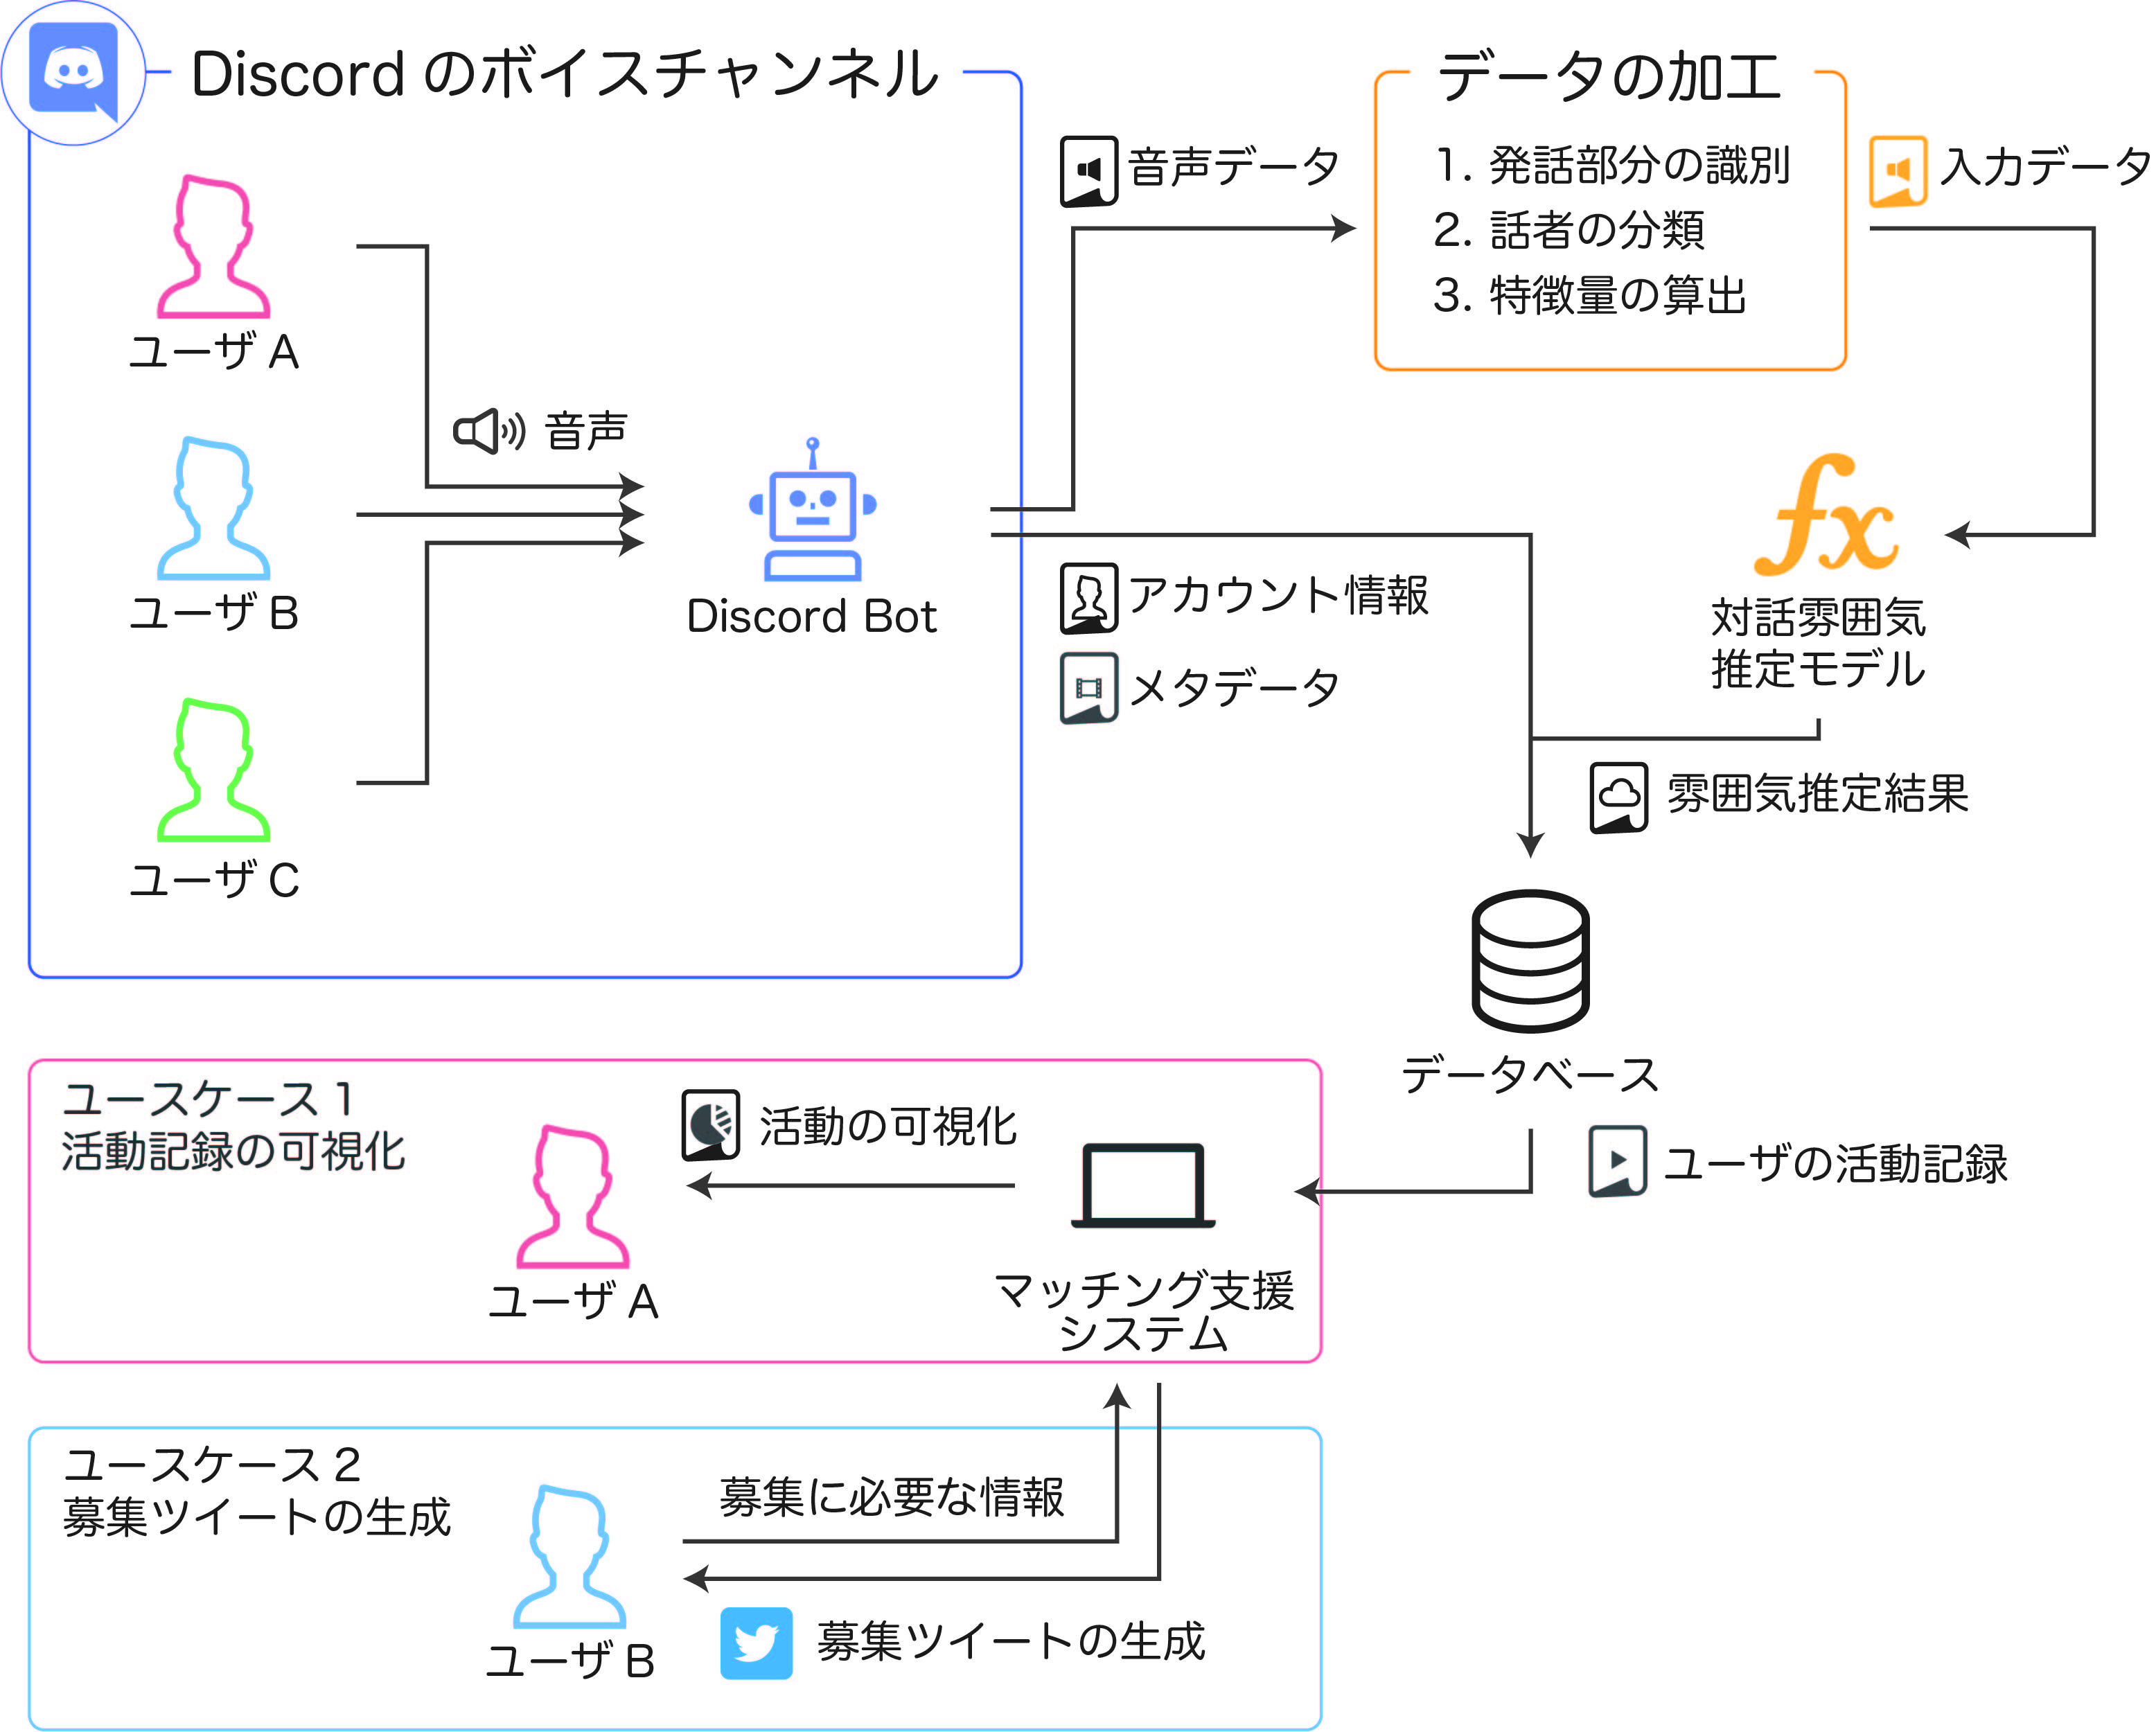
\includegraphics[width=0.95\textwidth]{figs/matching_system_big_arrow.jpg}
    }
    \caption{システムイメージ}
    \label{fig:matching_system_big_arrow}
\end{figure}

\section{対話雰囲気推定モジュール\label{node:estimation_module}}

本モジュールはDiscordで開催される作業通話を対象としており,作業通話の音声をBotによって収集し対話雰囲気の推定を行う.

\subsection{対話雰囲気推定モジュールで収集するデータ\label{item:estimation_module_collection_data}}

本モジュールは,対話雰囲気推定のために音声データの収集を行う.
その際には,第\ref{sec:related_researchs}章で述べた豊田らの手法を参考に,ユーザのプライバシーの担保や第\ref{sec:develop_estimation_model}章で述べる対話雰囲気推定モデルの構築における学習コストの低減を目的に限られた非言語情報のみを対象とする.
具体的には,どのユーザごとの発話時間情報(ユーザがいつどのくらいの時間発話したかの情報)と作業通話のメタデータのみを用いる.
作業通話のメタデータとしては,参加者のユーザ情報,開催時間情報が収集対象である.
また,収集した発話時間情報は特徴量として変換され対話雰囲気推定モデルの入力データとして対話雰囲気の推定に利用する.

\subsection{対話雰囲気推定モジュールで推定する雰囲気\label{item:estimated_atmosphere}}

本モジュールで推定を行う対話雰囲気は「盛り上がり」,「真面目さ」,「明るさ」,「くつろぎ」の四つである(表\ref{tab:estimation_definition}).
本研究のそれぞれの定義について述べる.

「盛り上がり」は対話の活発性を表現する雰囲気を指す.
「盛り上がり」が肯定の状態,つまり盛り上がっている雰囲気とは参加者同士のコミュニケーションが頻繁に行われており,相互行為が活発に行われている状態を指す.
反対に,「盛り上がり」が否定の状態,盛り下がっている,沈んでいる雰囲気とは参加者同士の会話や相互行為が少ない状態を指す.

「真面目さ」は対話の生産性や参加者が対話に熱心に取り組んでいるかを表現する雰囲気を指す.
「真面目さ」が肯定の状態,つまり真面目な雰囲気とは参加者が作業や議題に集中しており,生産性が高い状態を指す.
反対に,「真面目さ」が否定の状態,真面目でない,怠けている雰囲気とは参加者が雑談をしていたり,主目的とは別の言動を行なっている状態を指す.

「明るさ」は話題の内容や参加者の態度を表現する雰囲気を指す.
「明るさ」が肯定の状態,つまり明るい雰囲気とは話題がポジティブで,参加者が興奮している状態を指す.
反対に,「明るさ」が否定の状態,暗い,落ち着いた雰囲気とは話題がネガティブで,参加者が物事に対して否定的な状態を指す.

「くつろぎ」は参加への心理的安全性や対話への満足感を表現する雰囲気を指す.
「くつろぎ」が肯定の状態,つまりくつろいでいる雰囲気とは参加者同士の心理的安全性が高く,リラックスして参加できている状態を指す.
反対に,「くつろぎ」が否定の状態,気遣っている,緊張している雰囲気とは参加者がお互いの距離感や接し方がわからない状態や,物事に注視して集中している状態を指す.

これらの対話雰囲気は本研究独自で定義したものであり,参考にしている豊田らの定義した雰囲気とは異なる.
これは,豊田らは対面で行われる二者間の対話を対象としていることに対して,本研究では遠隔で行われる複数名での作業通話中の対話を対象としているためである.

これらの対話雰囲気の推定には機械学習を用いる.
具体的には対話雰囲気推定モデルを構築し,そのモデルによって入力された一つの対話における各雰囲気について肯定か否定の2値で推定を行う.
対話雰囲気推定モデルについては第\ref{sec:develop_estimation_model}章で詳細に述べる.

\begin{table}[t]
    \caption{推定を行う雰囲気}
    \centering
    \begin{tabular}{|l|l|l|l|}
        \hline
        名称 & 定義 & 肯定 & 否定 \\
        \hline\hline
        盛り上がり & 対話の活発性を表現 & 盛り上がっている & 沈んでいる \\
        \hline
        真面目さ & 対話の生産性や参加者が対話に & 真面目である & 怠けている \\
        & 熱心に取り組んでいるかを表現 & & \\
        \hline
        明るさ & 話題の内容や参加者の態度を表現 & 明るい & 暗い \\
        \hline
        くつろぎ  & 参加への心理的安全性や & くつろいでいる & 緊張している \\
        & 対話への満足感を表現 & & \\
        \hline
    \end{tabular}
    \label{tab:estimation_definition}
\end{table}

\subsection{対話雰囲気推定モジュールの利用方法}

対話雰囲気推定モジュールのユーザが操作を行う箇所はDiscord Botのみである.
本節ではDiscord Botの利用方法の想定を示す.
まず,Discord Botはユーザが作業通話を開催するサーバに招待されることで利用可能状態となる.
ユーザは作業通話を開始した際に開始用のコマンドをDiscord Botに対して入力することで録音を開始する.
また,ユーザは作業通話が終了した際に終了用のコマンドを入力.
終了用のコマンドを受信したDiscord Botは録音の停止と対話雰囲気の推定結果の出力をテキストチャンネル上に行う.
ユーザはDiscord Botにより出力された対話雰囲気の推定結果の確認や,主観的に正しいと感じた雰囲気への修正を行える.
それらのデータはデータベースに記録される.記録したデータは再び学習データとしてモデルの精度向上に利用されることを想定している.

\section{マッチング支援モジュール}

本モジュールは,第\ref{node:estimation_module}節のモジュールによってデータベースに記録されたデータを用いた二つのユースケースを想定した機能の実装をしている.

一つ目は,自身の活動記録や作業嗜好を客観的に確認したいというユースケースに向けた活動記録や作業嗜好の可視化機能である.
本機能は,ユーザの今まで開催した作業通話に関するデータを表示する(図\ref{fig:estimationgraph}).
表示する情報は,平均発話量,平均活動時間,一緒に活動する人,雰囲気それぞれについての傾向値である.
平均発話量の傾向値は,発話回数と発話時間を基に対象ユーザが無口であるか多弁であるかをスライダーで示す.
また,1分あたりの平均発話時間も併せて記載する.
平均活動時間の傾向値は,メタデータを基に平均活動時間長が短いか長いかをスライダーで示す.
また,作業通話を開催している時間帯の傾向についても併せて記載する.
一緒に活動する人の傾向値は,メタデータを基に作業通話を知人と初見どちらの人と開催することが多いかをスライダーで示す.
ここにおける知人とはDiscord上でフレンドになっているか,一度以上過去にともに作業通話を開催した記録がある人を指す.
雰囲気の傾向値とは盛り上がっている雰囲気の対話が多いことなどをレーダーチャートにて表現した値を示す.

\begin{figure}
    \centering
    \fbox{
        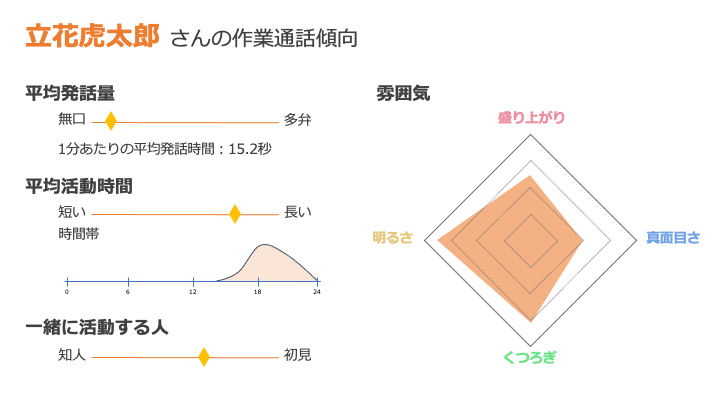
\includegraphics[width=0.7\textwidth]{figs/visualization.png}
    }
    \caption{作業嗜好の可視化イメージ}
    \label{fig:estimationgraph}
\end{figure}

二つ目は,効果的なSNS募集を行いたいというユースケースに向けた募集文(ツイート)の生成機能である.
本機能は,参加者を募りたい作業通話の概要を入力することで,その概要と一つ目の機能で可視化された自身のデータを掲載された募集文(ツイート)を生成し投稿する(図\ref{fig:tweet_image}).
本機能の対象は,Twitterで行われるSNS募集である.
本機能でユーザが入力する作業通話の概要情報は,作業内容,開催時間,募集人数の三つを想定している.
本機能は,一目で無縁ユーザ向けの募集文であることがわかることと,開催したい作業通話の概要がわかることによって明確で効率的な募集形態の実現を目指している.

\begin{figure}
    \centering
    \fbox{
        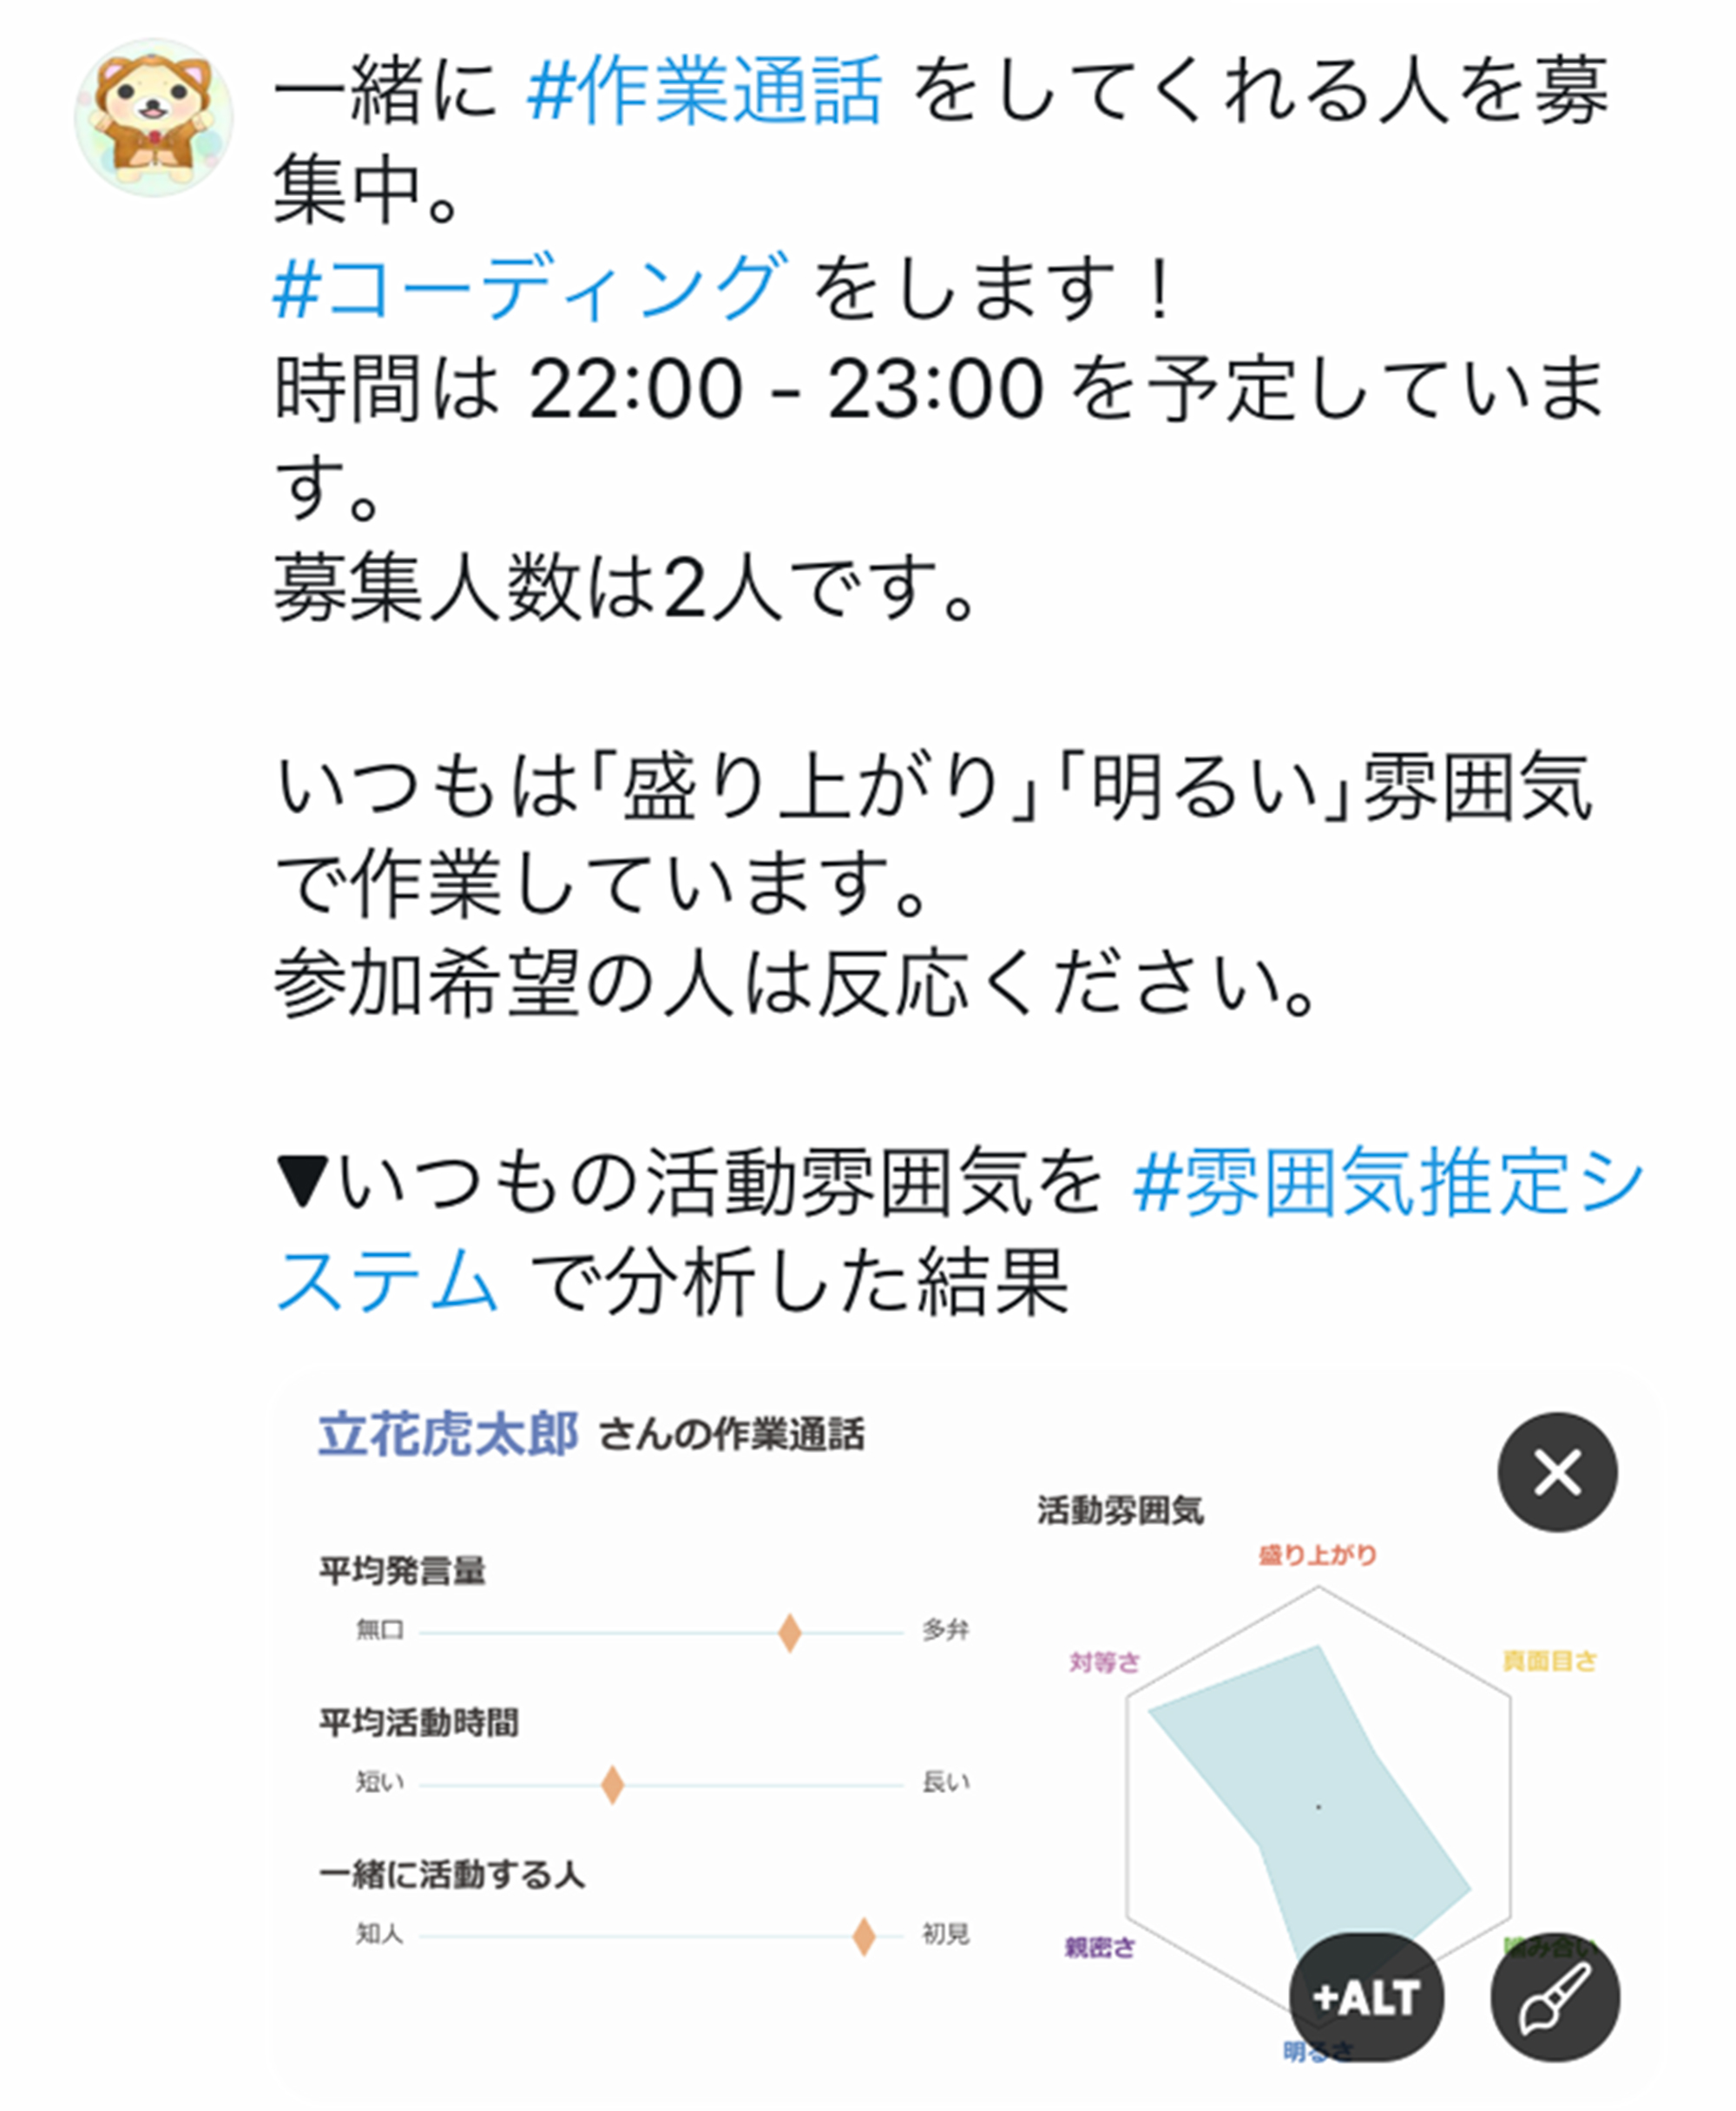
\includegraphics[width=0.7\textwidth]{figs/tweet_image.jpg}
    }
    \caption{生成する投稿のイメージ}
    \label{fig:tweet_image}
\end{figure}

将来的には,本モジュールを用いて作業嗜好の合うユーザの推薦等無縁ユーザとの繋がり形成の機会を増加させる機能の実装なども目指している.
結果として,SNS募集のデファクトスタンダードとなることでSNS募集の効率化と心理的負担の低下の実現を行えるモジュールを目指す.

\chapter{対話雰囲気推定モデルの構築\label{sec:develop_estimation_model}}
\thispagestyle{plain}

本研究では,機械学習によって通話中の音声から対話雰囲気を推定する.
本研究で構築する対話雰囲気推定モデルは,対話データから抽出した特徴量を入力値とし,第\ref{item:estimated_atmosphere}項で述べた各雰囲気について肯定,否定の2値での分類結果を出力値とする.
豊田らは二者対話を対象に発話時間特徴を特徴量とする機械学習を用いた対話雰囲気推定を行なっている\cite{Toyota}.
豊田らの構築したモデルは「盛り上がり」「まじめさ」「噛み合い」「明るさ」「親密さ」「対等さ」の6つの雰囲気を推定対象としており,それぞれ肯定,否定の2値で分類している.
特に「盛り上がり」「まじめさ」「親密さ」の推定においては全体正答率が0.8を超える高い値を示していることから,本研究でもこの手法に基づいて対話雰囲気推定モデルの構築を行う.
本章では,本研究における対話雰囲気推定モデルの構築手順について述べる.

\section{対話データの収集とラベル付け\label{node:deta_collection}}

学習データを構築するために対話データの収集を行う.
豊田らは対話データとして音声コーパス\cite{PASD}を採用している.
一方で,本研究では実際に開催された作業通話の録音データを採用する.
これは一般的な対話と作業通話中の対話はそれぞれ性質が異なるためである.
例えば,一般的な対話では沈黙は気まずく回避される傾向があるが,作業通話における沈黙は作業に集中していることの現れであり許容される傾向がある.
加えて,作業通話中の対話においては突発的な話題の変化が起こりやすく,独り言が行き交うことが多いなどの特徴がある.
このような作業通話中の対話の独特な性質が,対話雰囲気の形成に影響を与えていると十分に考えられることから,本研究では実際の作業通話の音声を学習に用いる.

対話データの収集とラベル付けの手順について述べる.
まず,対話データとして1 〜 4名の話者からなる計6時間弱の作業通話音声の録音を行う.
次に全ての音声を10 〜 120秒程度の対話になるように切り出す.
続いて,それぞれのデータに対して第\ref{item:estimated_atmosphere}項で述べた各雰囲気(「盛り上がり」,「真面目さ」,「明るさ」,「くつろぎ」)について主観で肯定か否定のラベル付けを行う.
ここで付与するラベルはのちの学習での教師ラベルとなる.
以上の手順により本研究では,計130対話を抽出しラベル付けされた対話データとした.

\section{発話状態集合の抽出}
% MEMO: 「発話集合」という表現がわかりにくい

特徴量の抽出を行うために,対話データから発話状態集合の抽出を行う.
発話状態集合とは,対話データにおける話者ごとの発話時間を発話状態ごとに記録した集合のことを指す.
豊田らの手法では,一つの対話データについて各話者の単独発話集合と二者の同時発話集合を抽出している.
この手法は二者の対話でのみ有効な抽出方法である.
しかし,本研究の手法における対象話者数は2 〜 4名であるため,異なる手法を用いて発話状態集合を抽出する.

はじめに,豊田らの手法は1名の話者のみが発話している状態を単独発話状態としてその集合を抽出しているが,本研究では他の話者の発話に依存せず話者ごとに発話している状態を発話集合として抽出する.
図\ref{fig:speaker_split}を例に述べる.
図\ref{fig:speaker_split}は対話データの一部を例として掲載しており,横軸が時間の流れを表している.
また,縦軸の各話者と同じ高さで引かれている線はそれぞれの話者が発話していることを表している.
図\ref{fig:speaker_split}において豊田らの手法の場合,話者$A$における単独発話集合は$\{3, 4, 3, 3, ...\}$となる.
一方本研究の場合,話者$A$における発話集合は$\{3, 5, 3, 3, ...\}$となる.

\begin{figure}
    \centering
    \fbox{
        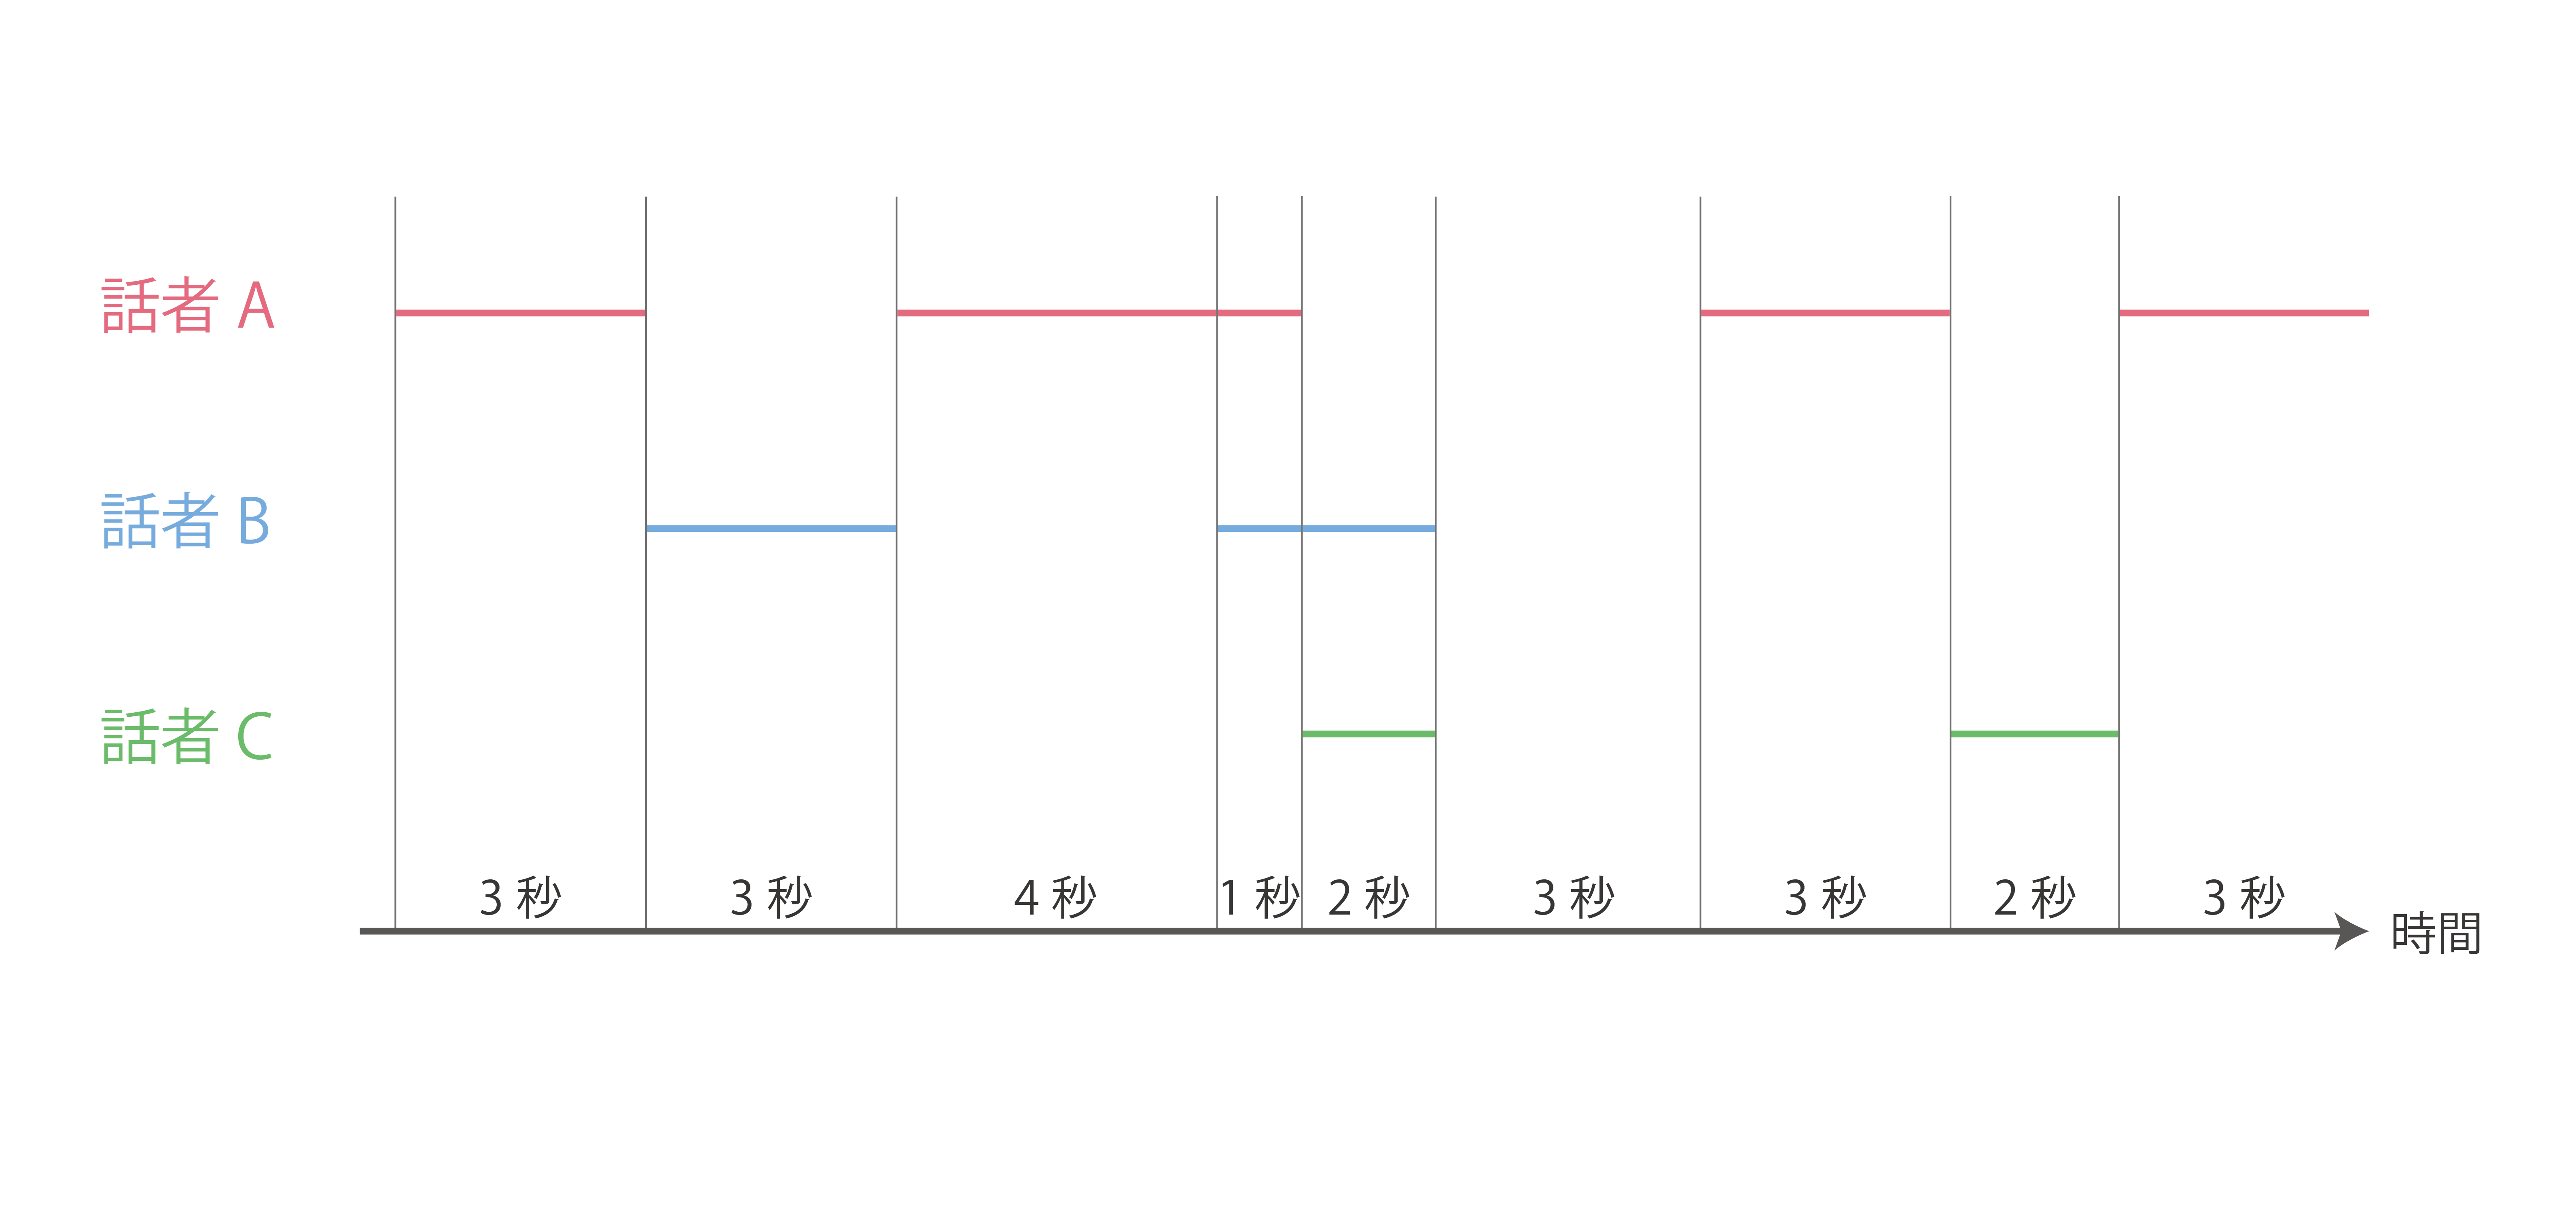
\includegraphics[width=0.7\textwidth]{figs/speaker_split.png}
    }
    \caption{対話データにおける発話の例}
    \label{fig:speaker_split}
\end{figure}

次に,豊田らの手法は二名の話者が同時に発話している状態を同時発話状態としてその集合を対話データにつき一つ抽出しているが,本研究では話者ごとに同時発話集合を抽出する.
図\ref{fig:speaker_split}において豊田らの手法の場合,同時発話集合は$\{1, 2, ...\}$となる.
一方本研究の場合,話者ごとに抽出するため話者$A$の同時発話集合は$\{1, ...\}$,話者$B$の同時発話集合は$\{1, 2, ...\}$,話者$C$の同時発話集合は$\{2, ...\}$となる.

以上が豊田らの手法で抽出した発話状態集合との比較である.
加えて本研究では,一つの対話データ全体としての傾向が対話雰囲気の形成に影響を与えていると仮定し,新たに三つの発話状態を定義しそれらの集合を抽出した.
一つ目は非発話状態である.
非発話状態は対話において一人も発話していない状態である.
非発話状態の集合である非発話集合は図\ref{fig:speaker_split}の場合,$\{3, ...\}$となる.
二つ目は全発話状態である.
全発話状態は全話者の発話状態を集約した発話状態である.
全発話状態の集合である全発話集合は図\ref{fig:speaker_split}の場合,$\{3, 5, 3, 3, 3, 3, 2, 2, ...\}$となる.
三つ目は全状態である.
全状態は全発話集合へ非発話状態を加えた状態である.
全状態の集合である全集合は図\ref{fig:speaker_split}の場合,$\{3, 5, 3, 3, 3, 3, 2, 2, 3 ...\}$となる.

以降,対話$d$におけて話者数は$n$,任意の発話状態集合は$S^d$と表現し,その集合における$i$番目の要素は$S^di$と表現する.
加えて,話者$x$についての発話集合は$S^d_{stx}$,同時発話集合は$S^d_{ssx}$と表現する.
また,同様に対話$d$に対する非発話集合は$S^d_{ns}$,全発話集合は$S^d_{us}$,全集合は$S^d_{as}$と表現する.

\section{特徴量の抽出\label{node:pickup_feature}}

抽出した発話状態集合から特徴量の抽出を行う.
豊田らは各集合に対する統計量とその統計量を比較した値(以下,「比較量」)を算出し特徴量としている.
本研究でも統計量と比較量を特徴量とするが,具体的に算出する値は異なる.

\subsection{統計量を用いた特徴量の抽出}

本研究で特徴量として採用する統計量とそれらの算出式を表\ref{tab:statistics_and_formulas}に示す.
本研究では,統計量としてそれぞれの集合に対する合計値,平均値,標準偏差,最大値,要素数,占有率を算出する.
それぞれの統計量の採用理由について述べる.
はじめに,合計値と平均値,要素数,占有率を計測することで話者の会話への積極性や興味の強さが対話雰囲気の形成に与える影響を測定するために採用した.
次に,標準偏差は話者間の発話の偏りが対話雰囲気の形成に与える影響を測定するために採用した.
最大値は対話における発話時間の値域が対話雰囲気の形成に与える影響を測定するために採用した.

\begingroup
\renewcommand{\arraystretch}{1.5}
\begin{table}[t]
    \caption{特徴量として採用する統計量と算出式}
    \centering
    \begin{tabular}{ll}
        \hline
        統計量 & 算出式 \\
        \hline\hline
        合計値 & $sum(S^d) = \sum_{i=1}^n S^di$ \\
        \hline
        平均値 & $mean(S^d) = \frac{sum(S^d)}{n}$ \\
        \hline
        標準偏差 & $std(S^d) = \sqrt{\frac{1}{n}\sum_{i=1}^n (S^di - mean(S^d))^2}$ \\
        \hline
        最大値 & $max(S^d) = \{r\in{S^d} | r \geq \forall{a}\in{S^d} \}$ \\
        \hline
        要素数  & $size(S^d) = |S^d|$ \\
        \hline
        占有率  & $share(S^d) = \frac{sum(S^d)}{sum(S^d_{as})}$ \\
        \hline
    \end{tabular}
    \label{tab:statistics_and_formulas}
\end{table}
\endgroup

\subsection{比較量を用いた特徴量の抽出}

統計量をもとに比較量を算出し特徴量とする.
本研究における二つの発話状態集合の比較量は,発話状態集合の各統計量について発話合計時間が短い方を長い方で除算することで算出する.
よって比較を行う発話状態集合両者に欠損値が存在しない場合は,一回の比較で6つの比較量が得られる.
本研究は比較量として話者間発話比較,話者間同時発話比較,他話者比較,話者内発話比較を算出する.
これらの比較量は各発話状態集合間で算出する.

はじめに,話者間発話比較は,対話$d$における任意の話者二名の発話状態を比較した値である.
話者間発話比較を求めることで,話者間の発話時間や発話頻度の比較を行うことができる.
これによって,対話における話者間のコミュニケーション量の違いが対話雰囲気の形成に与える影響を測定することができることから話者間発話比較を採用した.

次に,話者間同時発話比較は,対話$d$における任意の話者二名の同時発話状態を比較した値である.
話者間の発話量の比較について,二者の対話における同時発話状態の発生回数や占有率などの統計量が「盛り上がり」や「真面目さ」の対話雰囲気に影響を与えることが示唆されている\cite{Ito}\cite{Toyota}.
本研究では,同時発話集合を話者ごとに抽出しているため同様に同時発話状態の比較が対話雰囲気の推定に有効であると考え話者間同時発話比較を採用した.

続いて,他話者比較は,対話$d$における任意の話者一名と,その話者以外の話者の発話集合を結合させた集合を比較した値である.
他話者比較を求めることで,特定の話者だけでなく対話全体の中での発話時間や発話頻度を求め対象話者が聞き手であるか,話し手であるかを推定できる.
これにより,聞き手(話し手)の発話量が対話雰囲気に与える影響を測定できることから他話者比較を採用した.

話者内発話比較は,対話$d$における任意の話者一名の発話状態と同時発話状態を比較した値である.
話者内発話比較を求めることで,対話において一人の話者が一方的に発言を続けているかを推定することができる.
これにより,話者が他話者の発言をどの程度受け入れているかを測定できることから話者内発話比較を採用した.

\subsection{抽出する特徴量の一覧}

対話$d$について,本研究で抽出する特徴量を表\ref{tab:features_with_statistics}と表\ref{tab:features_with_comparative_quantities}に示す.
それぞれの表中の$x, y$は任意の話者を表現しており,$x$はより発話時間の合計値が高い話者を指している.
本研究で特徴量として算出される統計量,比較量の数は話者数に依存している.
抽出される特徴量数は,欠損値を含めると話者数2名で90個,話者数3名で144個,話者数4名で210個である.

\begin{table}[htpb]
  \caption{統計量を用いた特徴量}
  \centering
  \begin{tabular}{|c|c|c|}
      \hline
      特徴量番号 & 特徴量 & 算出式 \\\hline\hline
      $1_x$ & \multirow{6}{*}{話者$x$の発話集合に関する特徴量} & $sum(S^d_{stx})$ \\ \cline{1-1}\cline{3-3}
      $2_x$ & & $mean(S^d_{stx})$ \\ \cline{1-1}\cline{3-3}
      $3_x$ & & $std(S^d_{stx})$ \\ \cline{1-1}\cline{3-3}
      $4_x$ & & $max(S^d_{stx})$ \\ \cline{1-1}\cline{3-3}
      $5_x$ & & $size(S^d_{stx})$ \\ \cline{1-1}\cline{3-3}
      $6_x$ & & $share(S^d_{stx})$ \\ \hline
      $7_x$ & \multirow{6}{*}{話者$x$の同時発話集合に関する特徴量} & $sum(S^d_{ssx})$ \\ \cline{1-1}\cline{3-3}
      $8_x$ & & $mean(S^d_{ssx})$ \\ \cline{1-1}\cline{3-3}
      $9_x$ & & $std(S^d_{ssx})$ \\ \cline{1-1}\cline{3-3}
      $10_x$ & & $max(S^d_{ssx})$ \\ \cline{1-1}\cline{3-3}
      $11_x$ & & $size(S^d_{ssx})$ \\ \cline{1-1}\cline{3-3}
      $12_x$ & & $share(S^d_{ssx})$ \\ \hline
      $13$ & \multirow{6}{*}{非発話集合に関する特徴量} & $sum(S^d_{ns})$ \\ \cline{1-1}\cline{3-3}
      $14$ & & $mean(S^d_{ns})$ \\ \cline{1-1}\cline{3-3}
      $15$ & & $std(S^d_{ns})$ \\ \cline{1-1}\cline{3-3}
      $16$ & & $max(S^d_{ns})$ \\ \cline{1-1}\cline{3-3}
      $17$ & & $size(S^d_{ns})$ \\ \cline{1-1}\cline{3-3}
      $18$ & & $share(S^d_{ns})$ \\ \hline
      $13$ & \multirow{6}{*}{全発話集合に関する特徴量} & $sum(S^d_{us})$ \\ \cline{1-1}\cline{3-3}
      $14$ & & $mean(S^d_{us})$ \\ \cline{1-1}\cline{3-3}
      $15$ & & $std(S^d_{us})$ \\ \cline{1-1}\cline{3-3}
      $16$ & & $max(S^d_{us})$ \\ \cline{1-1}\cline{3-3}
      $17$ & & $size(S^d_{us})$ \\ \cline{1-1}\cline{3-3}
      $18$ & & $share(S^d_{us})$ \\ \hline
      $13$ & \multirow{6}{*}{全集合に関する特徴量} & $sum(S^d_{as})$ \\ \cline{1-1}\cline{3-3}
      $14$ & & $mean(S^d_{as})$ \\ \cline{1-1}\cline{3-3}
      $15$ & & $std(S^d_{as})$ \\ \cline{1-1}\cline{3-3}
      $16$ & & $max(S^d_{as})$ \\ \cline{1-1}\cline{3-3}
      $17$ & & $size(S^d_{as})$ \\ \cline{1-1}\cline{3-3}
      $18$ & & $share(S^d_{as})$ \\ \hline
  \end{tabular}
  \label{tab:features_with_statistics}
\end{table}

\begin{table}[htpb]
    \caption{比較量を用いた特徴量}
    \centering
    \begin{tabular}{|c|c|c|}
        \hline
        特徴量番号 & 特徴量 & 算出式 \\ \hline\hline
        $19_{xy}$ & \multirow{6}{*}{話者$x, y$の話者間発話比較に関する特徴量} & $\frac{sum(S^d_{sty})}{sum(S^d_{stx})}$ \\ \cline{1-1}\cline{3-3}
        $20_{xy}$ & & $\frac{mean(S^d_{sty})}{mean(S^d_{stx})}$ \\ \cline{1-1}\cline{3-3}
        $21_{xy}$ & & $\frac{std(S^d_{sty})}{std(S^d_{stx})}$ \\ \cline{1-1}\cline{3-3}
        $22_{xy}$ & & $\frac{max(S^d_{sty})}{max(S^d_{stx})}$ \\ \cline{1-1}\cline{3-3}
        $23_{xy}$ & & $\frac{size(S^d_{sty})}{size(S^d_{stx})}$ \\ \cline{1-1}\cline{3-3}
        $24_{xy}$ & & $\frac{share(S^d_{sty})}{share(S^d_{stx})}$ \\ \hline
        $25_{xy}$ & \multirow{6}{*}{話者$x, y$の話者間同時発話比較に関する特徴量} & $\frac{sum(S^d_{ssy})}{sum(S^d_{ssx})}$ \\ \cline{1-1}\cline{3-3}
        $26_{xy}$ & & $\frac{mean(S^d_{ssy})}{mean(S^d_{ssx})}$ \\ \cline{1-1}\cline{3-3}
        $27_{xy}$ & & $\frac{std(S^d_{ssy})}{std(S^d_{ssx})}$ \\ \cline{1-1}\cline{3-3}
        $28_{xy}$ & & $\frac{max(S^d_{ssy})}{max(S^d_{ssx})}$ \\ \cline{1-1}\cline{3-3}
        $29_{xy}$ & & $\frac{size(S^d_{ssy})}{size(S^d_{ssx})}$ \\ \cline{1-1}\cline{3-3}
        $30_{xy}$ & & $\frac{share(S^d_{ssy})}{share(S^d_{ssx})}$ \\ \hline
        $31_{x}$ & \multirow{6}{*}{話者$x$の他話者発話比較に関する特徴量} & $\frac{sum(S^d_{stx})}{sum(\overline{S^d_{stx}} \cap S^d_{us})}$ \\ \cline{1-1}\cline{3-3}
        $32_{x}$ & & $\frac{mean(S^d_{stx})}{mean(\overline{S^d_{stx}} \cap S^d_{us})}$ \\ \cline{1-1}\cline{3-3}
        $33_{x}$ & & $\frac{std(S^d_{stx})}{std(\overline{S^d_{stx}} \cap S^d_{us})}$ \\ \cline{1-1}\cline{3-3}
        $34_{x}$ & & $\frac{max(S^d_{stx})}{max(\overline{S^d_{stx}} \cap S^d_{us})}$ \\ \cline{1-1}\cline{3-3}
        $35_{x}$ & & $\frac{size(S^d_{stx})}{size(\overline{S^d_{stx}} \cap S^d_{us})}$ \\ \cline{1-1}\cline{3-3}
        $36_{x}$ & & $\frac{share(S^d_{stx})}{share(\overline{S^d_{stx}} \cap S^d_{us})}$ \\ \hline
        $37_{x}$ & \multirow{6}{*}{話者$x$の話者内発話比較に関する特徴量} & $\frac{sum(S^d_{stx})}{sum(S^d_{ssx})}$ \\ \cline{1-1}\cline{3-3}
        $38_{x}$ & & $\frac{mean(S^d_{stx})}{mean(S^d_{ssx})}$ \\ \cline{1-1}\cline{3-3}
        $39_{x}$ & & $\frac{std(S^d_{stx})}{std(S^d_{ssx})}$ \\ \cline{1-1}\cline{3-3}
        $40_{x}$ & & $\frac{max(S^d_{stx})}{max(S^d_{ssx})}$ \\ \cline{1-1}\cline{3-3}
        $41_{x}$ & & $\frac{size(S^d_{stx})}{size(S^d_{ssx})}$ \\ \cline{1-1}\cline{3-3}
        $42_{x}$ & & $\frac{share(S^d_{stx})}{share(S^d_{ssx})}$ \\ \hline
    \end{tabular}
    \label{tab:features_with_comparative_quantities}
\end{table}
  

\section{学習\label{node:machine_learning}}

本研究で構築する対話雰囲気推定モデルは,対象とする雰囲気や話者数が豊田らと異なるため一部独自の手法を採用する.
本研究では,対象雰囲気,対象話者数ごとに計12種の対話雰囲気推定モデルの構築を行う.
これは対象となる雰囲気や話者数によって有効な特徴量が異なるという仮説に基づいているためである.

本研究では,学習の前に学習データの前処理を行う.
具体的には,学習する対話雰囲気推定モデルの話者数によって欠損値を含む特徴量と学習データの削除を行う.
話者数3名を対象とする対話雰囲気推定モデルの学習を例とする.
まず,特徴量の削減を行う.
削減の対象となる特徴量は,話者3名を対象としたモデルでは不要となる話者数4名の場合に抽出される特徴量である.
具体的には,表\ref{tab:features_with_statistics}における特徴量番号$1$の4者目の特徴量や,表\ref{tab:features_with_comparative_quantities}における特徴量番号$19$の4者目を比較対象とする特徴量などである.
続いて,学習データの削除を行う.
削除の対象となる学習データは,話者3名を対象としたモデルでは不要となる話者数2名による学習データである.
これは話者数2名の学習データは,特徴量番号$1$の3者目の特徴量や特徴量番号$19$の3者目を比較対象とする特徴量など話者数に依存した特徴量が算出できず欠損値が発生するためである.

前処理を行ったものを最終的な学習データとして学習を行う.
学習を行う際に定める必要のある設定を表\ref{tab:learning_setting}に示す.
対象雰囲気は第\ref{item:estimated_atmosphere}項で述べた「盛り上がり」,「真面目さ」,「明るさ」,「くつろぎ」の4つから選択する.
対象話者数は2 〜 4名から選択する.
学習モデルは,どの学習モデルが本研究の学習において有効であるか比較を行うためLinear SVC,k近傍法,SVC,Naïve Bayesの4つを採用する.

\begin{table}[t]
    \caption{学習の設定}
    \centering
    \begin{tabular}{ll}
        \hline
        設定項目 & 範囲・候補 \\ \hline\hline
        \multirow{4}{*}{対象雰囲気} & 盛り上がり \\
        & 真面目さ \\
        & 明るさ \\
        & くつろぎ \\ \hline
        対象話者数 & 2 〜 4 \\ \hline
        \multirow{4}{*}{学習アルゴリズム} & Linear SVC \\
        & k近傍法 \\
        & SVC \\
        & Naive Bayes \\ \hline
    \end{tabular}
    \label{tab:learning_setting}
\end{table}

\section{特徴量選択\label{node:ga}}

第\ref{node:machine_learning}節で述べた設定を行うことで対話雰囲気推定モデルを構築することができる.
しかし,一般に多変量解析において解析に用いる特徴量が多くなると特徴空間が広がることで学習効率が低下する問題が知られている.
本研究で構築する対話雰囲気推定モデルでは最大210個の特徴量を用いるため,数ある特徴量の中から対話雰囲気の推定に有効な特徴量のみを用いて学習することで精度や学習速度の向上が見込める.
そこで本研究は特徴量選択を行う.
特徴量選択の手法は,豊田らにならい遺伝的アルゴリズム(以下,「GA」)を採用する.
GAでは特徴量数と同じ長さのビット列からなる染色体を生成し,各特徴量の利用有無を1:有効,0:無効で表現する.
GAの設定を表\ref{tab:ga_setting}に示す.
表中の個体評価における選択特徴量数とモデル正答率の重み付け和による評価は以下の式によって算出する.
式中の$W$は正答率と選択特徴量数の重み付けを表現しており,$[0, 1]$の値をとる.

\begin{equation}
    評価値 = \frac{正答数}{検証データ数} W + (1 - \frac{選択特徴量数}{全特徴量数}) (1 - W)
\end{equation}

\begin{table}[t]
    \caption{遺伝的アルゴリズムの設定}
    \centering
    \begin{tabular}{ll}
        \hline
        設定項目 & 範囲・候補 \\ \hline\hline
        \multirow{2}{*}{交叉方法} & 二点交叉 \\
        & 一様交叉 \\ \hline
        集団の大きさ & 100 / 300 / 1000 \\ \hline
        染色体突然変異率 & 0.0 〜 0.5 \\ \hline
        遺伝子突然変異率 & 0.0 〜 0.5 \\ \hline
        \multirow{3}{*}{個体評価方法} & モデル正答率による単純評価 \\
        & 選択特徴量数とモデル正答率の重み付け和による単純評価 \\
        & 選択特徴量数とモデル正答率の重み付け和による交差検証 \\ \hline
        選択方法 & エリート選択 \\ \hline
        エリート染色体選択数 & 10 / 30 / 1000 \\ \hline
        世代数 & 100 / 250 / 1000 \\ \hline
    \end{tabular}
    \label{tab:ga_setting}
\end{table}

\chapter{学習結果と考察\label{sec:evaluate_estimation_model}}
\thispagestyle{plain}

本章では,第\ref{sec:develop_estimation_model}章で述べた手法で構築した対話雰囲気推定モデルの学習結果と考察について述べる.
はじめに,本研究における対話雰囲気推定モデルの評価手法について述べる.
次に,特徴量選択を用いない対話雰囲気推定モデルの学習結果について述べる.
続いて,特徴量選択を用いた学習の比較基となるベースモデルについて述べる.
最後に,ベースモデルを中心に特徴量選択を用いた学習の結果について述べる.

\section{評価手法}

本研究における対話雰囲気推定モデルの評価はモデル正答率と選択特徴量数を用いる.
これはモデル正答率が高いほど正確な推定が期待でき,選択特徴量数が少ないほど軽量な推定が期待できるためである.
また,モデル評価は第\ref{node:ga}節で述べた個体評価とは異なり,二つの評価観点を一つの評価値と算出することはしない.
これは豊田らの手法においても同様の手法を用いていることと,どちらの観点が重要視されるべきか十分に検討できていないためである.
評価手法の検討については考察で詳細を述べる.

\section{特徴量選択を用いない対話雰囲気推定モデルの学習結果\label{node:learning_result_without_ga}}

対話雰囲気推定モデルの学習における特徴量選択の有効性の評価を行うために,特徴量選択を用いない対話雰囲気推定モデルの構築を行う.
特徴量選択を用いない対話雰囲気推定モデルの学習結果を表\ref{tab:excitement_learning_result_without_FS} 〜 表\ref{tab:comfortable_learning_result_without_FS}に示す.
特徴量選択を用いない対話雰囲気推定モデルは各対象雰囲気,対象話者数,学習モデルを網羅的に組み合わせて構築した.
表中のモデル正答率は有効数字4桁で,小数点第4位を四捨五入したものを掲載している.
いずれにおいても特徴量選択は行なっていないため,学習に利用した特徴量は話者数に依存した最大値となっている.

学習結果から明らかになったことについて述べる.
学習アルゴリズムはいずれの対象雰囲気のモデルにおいても対象話者数が2名または3名の場合,Naive Bayesのモデル正答率が高いことが明らかになった.
一方で,対象話者数が4名のモデルにおけるモデル正答率はモデル番号33の0.300など極端に低い値であるものも確認できる.
また,豊田らの構築した対話雰囲気推定モデルはモデル正答率が0.700 〜 0.855であったことから,これらのモデルのモデル正答率が低いことがわかる.

\begin{table}[ptb]
    \caption{「盛り上がり」を対象とした特徴量選択を用いない学習の結果}
    \centering
    \begin{tabular}{|c|c|l|r|c|}
        \hline
        モデル番号 & 対象話者数 & 学習アルゴリズム & モデル正答率 & 選択特徴量数 \\\hline\hline
        1 & \multirow{4}{*}{2} & Linear SVC & 0.6240 & \multirow{4}{*}{90} \\ \cline{1-1}\cline{3-4}
        2 & & k近傍法 & 0.6400 & \\ \cline{1-1}\cline{3-4}
        3 & & SVC & 0.7040 & \\ \cline{1-1}\cline{3-4}
        4 & & Naive Bayes & 0.7440 & \\ \hline
        5 & \multirow{4}{*}{3} & Linear SVC & 0.4699 & \multirow{4}{*}{144} \\ \cline{1-1}\cline{3-4}
        6 & & k近傍法 & 0.5772 & \\ \cline{1-1}\cline{3-4}
        7 & & SVC & 0.6515 & \\ \cline{1-1}\cline{3-4}
        8 & & Naive Bayes & 0.6632 & \\ \hline
        9 & \multirow{4}{*}{4} & Linear SVC & 0.3300 & \multirow{4}{*}{210} \\ \cline{1-1}\cline{3-4}
        10 & & k近傍法 & 0.5900 & \\ \cline{1-1}\cline{3-4}
        11 & & SVC & 0.6200 & \\ \cline{1-1}\cline{3-4}
        12 & & Naive Bayes & 0.4800 & \\ \hline
    \end{tabular}
    \label{tab:excitement_learning_result_without_FS}
\end{table}

\begin{table}[tpb]
    \caption{「真面目さ」を対象とした特徴量選択を用いない学習の結果}
    \centering
    \begin{tabular}{|c|c|l|r|c|}
        \hline
        モデル番号 & 対象話者数 & 学習アルゴリズム & モデル正答率 & 選択特徴量数 \\\hline\hline
        13 & \multirow{4}{*}{2} & Linear SVC & 0.6362 & \multirow{4}{*}{90} \\ \cline{1-1}\cline{3-4}
        14 & & k近傍法 & 0.4676 & \\ \cline{1-1}\cline{3-4}
        15 & & SVC & 0.5486 & \\ \cline{1-1}\cline{3-4}
        16 & & Naive Bayes & 0.6610 & \\ \hline
        17 & \multirow{4}{*}{3} & Linear SVC & 0.4222 & \multirow{4}{*}{144} \\ \cline{1-1}\cline{3-4}
        18 & & k近傍法 & 0.4417 & \\ \cline{1-1}\cline{3-4}
        19 & & SVC & 0.5583 & \\ \cline{1-1}\cline{3-4}
        20 & & Naive Bayes & 0.6028 & \\ \hline
        21 & \multirow{4}{*}{4} & Linear SVC & 0.5000 & \multirow{4}{*}{210} \\ \cline{1-1}\cline{3-4}
        22 & & k近傍法 & 0.7000 & \\ \cline{1-1}\cline{3-4}
        23 & & SVC & 0.5000 & \\ \cline{1-1}\cline{3-4}
        24 & & Naive Bayes & 0.6000 & \\ \hline
    \end{tabular}
    \label{tab:seriousness_learning_result_without_FS}
\end{table}

\begin{table}[ptb]
    \caption{「明るさ」を対象とした特徴量選択を用いない学習の結果}
    \centering
    \begin{tabular}{|c|c|l|r|c|}
        \hline
        モデル番号 & 対象話者数 & 学習アルゴリズム & モデル正答率 & 選択特徴量数 \\\hline\hline
        25 & \multirow{4}{*}{2} & Linear SVC & 0.5638 & \multirow{4}{*}{90} \\ \cline{1-1}\cline{3-4}
        26 & & k近傍法 & 0.5057 & \\ \cline{1-1}\cline{3-4}
        27 & & SVC & 0.5629 & \\ \cline{1-1}\cline{3-4}
        28 & & Naive Bayes & 0.7181 & \\ \hline
        29 & \multirow{4}{*}{3} & Linear SVC & 0.6722 & \multirow{4}{*}{144} \\ \cline{1-1}\cline{3-4}
        30 & & k近傍法 & 0.5306 & \\ \cline{1-1}\cline{3-4}
        31 & & SVC & 0.5389 & \\ \cline{1-1}\cline{3-4}
        32 & & Naive Bayes & 0.7000 & \\ \hline
        33 & \multirow{4}{*}{4} & Linear SVC & 0.3000 & \multirow{4}{*}{210} \\ \cline{1-1}\cline{3-4}
        34 & & k近傍法 & 0.7000 & \\ \cline{1-1}\cline{3-4}
        35 & & SVC & 0.6000 & \\ \cline{1-1}\cline{3-4}
        36 & & Naive Bayes & 0.4000 & \\ \hline
    \end{tabular}
    \label{tab:cheerfulness_learning_result_without_FS}
\end{table}

\begin{table}[tpb]
    \caption{「くつろぎ」を対象とした特徴量選択を用いない学習の結果}
    \centering
    \begin{tabular}{|c|c|l|r|c|}
        \hline
        モデル番号 & 対象話者数 & 学習アルゴリズム & モデル正答率 & 選択特徴量数 \\\hline\hline
        37 & \multirow{4}{*}{2} & Linear SVC & 0.6200 & \multirow{4}{*}{90} \\ \cline{1-1}\cline{3-4}
        38 & & k近傍法 & 0.5924 & \\ \cline{1-1}\cline{3-4}
        39 & & SVC & 0.5210 & \\ \cline{1-1}\cline{3-4}
        40 & & Naive Bayes & 0.6648 & \\ \hline
        41 & \multirow{4}{*}{3} & Linear SVC & 0.5778 & \multirow{4}{*}{144} \\ \cline{1-1}\cline{3-4}
        42 & & k近傍法 & 0.5806 & \\ \cline{1-1}\cline{3-4}
        43 & & SVC & 0.5583 & \\ \cline{1-1}\cline{3-4}
        44 & & Naive Bayes & 0.7000 & \\ \hline
        45 & \multirow{4}{*}{4} & Linear SVC & 0.6000 & \multirow{4}{*}{210} \\ \cline{1-1}\cline{3-4}
        46 & & k近傍法 & 0.5000 & \\ \cline{1-1}\cline{3-4}
        47 & & SVC & 0.6000 & \\ \cline{1-1}\cline{3-4}
        48 & & Naive Bayes & 0.7000 & \\ \hline
    \end{tabular}
    \label{tab:comfortable_learning_result_without_FS}
\end{table}


\section{ベースモデルの決定\label{node:base_model}}

本研究では,第\ref{node:machine_learning}節と第\ref{node:ga}節で示した各設定値を定めた上で学習を行う.
そこで,特徴選択を行うにあたって各設定値の学習効率への影響を容易に比較するために,比較基となるベースモデルを定める(表\ref{tab:base_model_setting}).
ベースモデルの対象雰囲気は「盛り上がり」とする.
これは豊田らの手法と本研究における推定対象の雰囲気を比較した際に,同一の定義を行っていることに加え,豊田らの研究におけるモデル正答率が0.855と高水準であるためである.
続いて対象話者数は3名とする.
これには二つの理由がある.
一つ目は,豊田らの手法と異なり三者以上の話者を対象とした対話雰囲気推定モデルを構築していることが本研究の独自性の一つであることから,三者以上の話者を対象としたモデルを比較の中心にすることが妥当であると考えたためである.
二つ目は,対象話者数が4名の学習データは第\ref{node:machine_learning}節で述べた前処理を行った結果,学習に用いることができるデータ数が3名に比較し必ず少なくなることから,対象話者数が増加することでモデルの信憑性が低下するためである.
学習アルゴリズムはNaive Bayesを採用する.
これは特徴量選択を行わない学習では,Naive Bayesが最も良いモデル正答率を持っているためである.
それ以降の特徴量選択に関わる設定は,事前に何度か無作為に設定を定めて学習をした上で最もモデル正答率が高く,選択特徴量数が少ないものを採用する.
その際の,評価における重み付け$W$は0.5である.
以上のベースモデルを用いて各学習設定や特徴量選択の有効性を評価する.

\begin{table}[t]
    \caption{ベースモデルの設定値}
    \centering
    \begin{tabular}{ll}
        \hline
        設定項目 & 範囲・候補 \\ \hline\hline
        対象雰囲気 & 盛り上がり \\ \hline
        対象話者数 & 3 \\ \hline
        学習アルゴリズム & Naive Bayes \\ \hline
        交叉方法 & 一様交叉 \\ \hline
        集団の大きさ & 100 \\ \hline
        染色体突然変異率 & 0.05 \\ \hline
        遺伝子突然変異率 & 0.10 \\ \hline
        個体評価方法 & 選択特徴量数とモデル正答率の重み付け和による交差検証 \\ \hline
        選択方法 & エリート選択 \\ \hline
        エリート染色体選択数 & 10 \\ \hline
        世代数 & 250 \\ \hline
    \end{tabular}
    \label{tab:base_model_setting}
\end{table}

\section{特徴量選択を用いた対話雰囲気推定モデルの学習結果\label{node:learning_result_with_ga}}

第\ref{node:base_model}節で述べたベースモデルを基に特徴量選択を用いた対話雰囲気推定モデルを構築する.
はじめに,ベースモデルから対象雰囲気,話者数を変更したモデルについて述べ,続いて特徴量選択の各設定を変更したモデルについて述べる.

\subsection{対象雰囲気,話者数を変更したモデルの学習結果\label{item:learning_result_with_ga_change_targets}}

ベースモデルとベースモデルから対象雰囲気,話者数を変更した全てのモデルの学習結果の一例を表\ref{tab:learn_result_with_ga}に示す.
表中のモデル番号50がベースモデルを表している.

\begin{table}[t]
    \caption{特徴量選択を用いたモデルの学習結果}
    \centering
    \begin{tabular}{|c|c|c|r|r|}
        \hline
        モデル番号 & 対象雰囲気 & 対象話者数 & モデル正答率 & 選択特徴量数 \\
        \hline\hline
        49 & \multirow{3}{*}{盛り上がり} & 2 & 0.800 & 10 \\ \cline{1-1}\cline{3-5}
        50 & & 3 & 0.795 & 21 \\ \cline{1-1}\cline{3-5}
        51 & & 4 & 0.860 & 45 \\ \hline
        52 & \multirow{3}{*}{真面目さ} & 2 & 0.775 & 16 \\ \cline{1-1}\cline{3-5}
        53 & & 3 & 0.769 & 30 \\ \cline{1-1}\cline{3-5}
        54 & & 4 & 0.800 & 38 \\ \hline
        55 & \multirow{3}{*}{明るさ} & 2 & 0.830 & 12 \\ \cline{1-1}\cline{3-5}
        56 & & 3 & 0.863 & 33 \\ \cline{1-1}\cline{3-5}
        57 & & 4 & 0.700 & 40 \\ \hline
        58 & \multirow{3}{*}{くつろぎ} & 2 & 0.790 & 13 \\ \cline{1-1}\cline{3-5}
        59 & & 3 & 0.816 & 25 \\ \cline{1-1}\cline{3-5}
        60 & & 4 & 0.900 & 40 \\ \hline
    \end{tabular}
    \label{tab:learn_result_with_ga}
\end{table}

この結果から明らかになったことについて述べる.

はじめに,ベースモデルに着目する.
特徴量選択を行う前のベースモデルと同条件のモデルは表\ref{tab:excitement_learning_result_without_FS}のモデル番号8である.
これらのモデルを比較するとモデル正答率が0.663から0.795に向上し,選択特徴量数が144から21に減少していることが確認できる.
ベースモデルの学習過程を図\ref{fig:exc3_crossover}に示す.
図\ref{fig:exc3_crossover}は横軸がGAの世代数を表しており,オレンジ色の値がモデル正答率,緑色の値が全体に対する選択特徴量数の割合,青色が評価値を表している.
図\ref{fig:exc3_crossover}からも学習が進むにつれてモデル正答率と選択特徴量数が変化していることがわかる.

\begin{figure}
    \centering
    \fbox{
        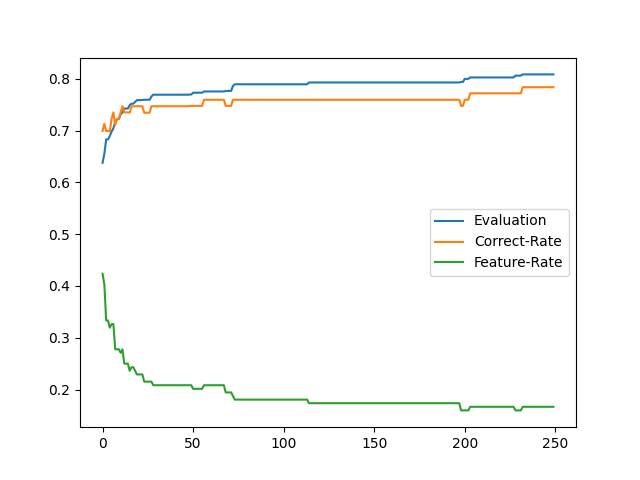
\includegraphics[width=0.7\textwidth]{figs/exc3_crossover.png}
    }
    \caption{ベースモデルの学習過程}
    \label{fig:exc3_crossover}
\end{figure}

次に,全体のモデル正答率に着目する.
ベースモデル同様,全体としてモデル正答率の向上を確認できる.
事実,表\ref{tab:excitement_learning_result_without_FS} 〜 表\ref{tab:comfortable_learning_result_without_FS}のうちNaive Bayesを学習モデルとして採用しているモデルと,表\ref{tab:learn_result_with_ga}のモデルのモデル正答率について両側5%のt検定を行った結果,P値が$3.5727 \times 10^{-5}$を示すことから有意差を確認できる(表\ref{tab:correct_rate_t-test}).
豊田らの構築した対話雰囲気推定モデルの正答率と比較しても大きな差は見られず同程度の精度を持つモデルであることがわかる.
また,対象雰囲気間によるモデル正答率の差は小さいことが確認できる.
一方で,話者数の増加に伴ってモデル正答率が不安定になっていることが確認できる.
特に,対象話者が4名の場合は顕著である(図\ref{fig:exc4} 〜 図\ref{fig:com4}).

\begin{table}[t]
    \caption{特徴量選択前後のモデル正答率のt検定}
    \centering
    \begin{tabular}{cc}
        \hline
        算出項目 & 算出値 \\
        \hline\hline
        \multirow{2}{*}{平均値} & 特徴量選択前: $0.6362$ \\
        & 特徴量選択後: $0.8085$ \\ \hline
        \multirow{2}{*}{分散値} & 特徴量選択前: $0.0105$ \\
        & 特徴量選択後: $0.0027$ \\ \hline
        t値 & $-6.6579$ \\ \hline
        t境界値 & $2.2010$ \\ \hline
        P値 & $3.5727 \times 10^{-5}$ \\ \hline
    \end{tabular}
    \label{tab:correct_rate_t-test}
\end{table}

\begin{figure}
    \centering
    \fbox{
        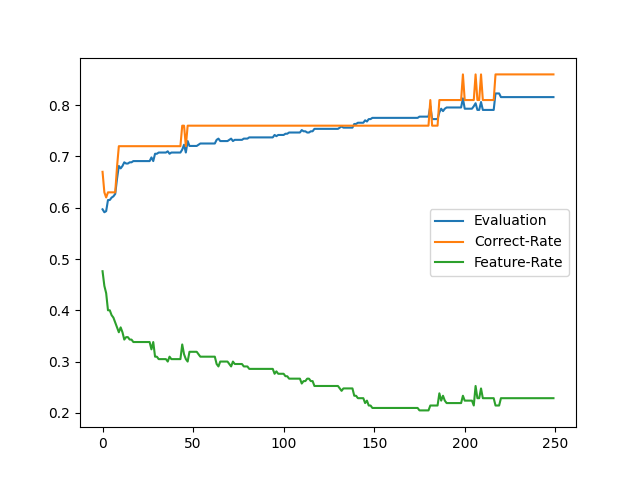
\includegraphics[width=0.7\textwidth]{figs/exc4.png}
    }
    \caption{「盛り上がり」話者数4名のモデル学習過程}
    \label{fig:exc4}
\end{figure}

\begin{figure}
    \centering
    \fbox{
        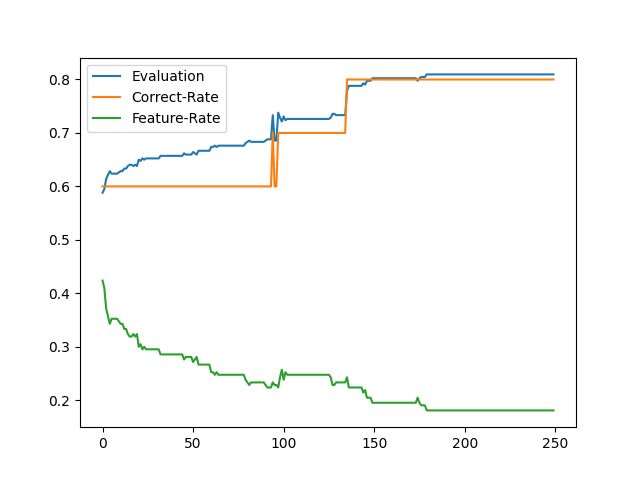
\includegraphics[width=0.7\textwidth]{figs/ser4.png}
    }
    \caption{「真面目さ」話者数4名のモデル学習過程}
    \label{fig:ser4}
\end{figure}

\begin{figure}
    \centering
    \fbox{
        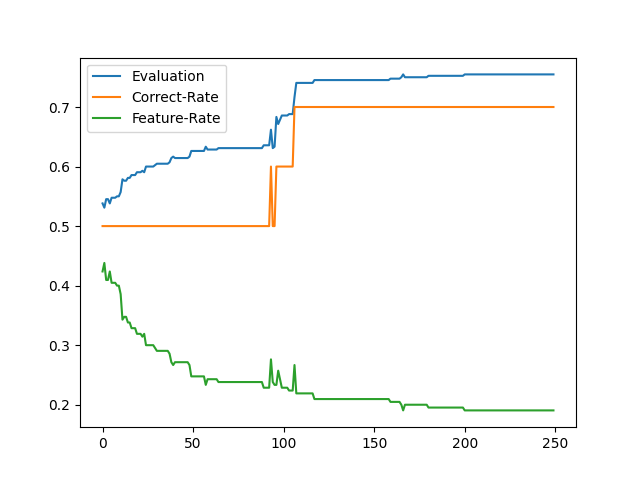
\includegraphics[width=0.7\textwidth]{figs/che4.png}
    }
    \caption{「明るさ」話者数4名のモデル学習過程}
    \label{fig:che4}
\end{figure}

\begin{figure}
    \centering
    \fbox{
        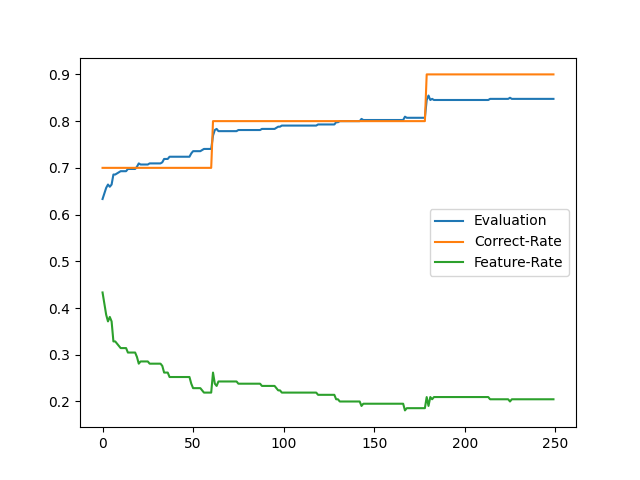
\includegraphics[width=0.7\textwidth]{figs/com4.png}
    }
    \caption{「くつろぎ」話者数4名のモデル学習過程}
    \label{fig:com4}
\end{figure}

最後に選択特徴量数に着目する.
全ての対象雰囲気において対象話者数の増加に伴って,選択特徴量数の増加を確認できる.
一方で,同じ対象話者数のモデルを対象雰囲気間で比較しても大きな差は確認できない.
また,選択特徴量数とモデル正答率においても本結果からは相関を確認することはできない.

\subsection{特徴量選択の設定を変更したモデルの学習結果\label{item:learning_result_with_ga_change_params}}

ベースモデから特徴量選択の各設定を変更した対話雰囲気推定モデルの学習結果の一部を表\ref{tab:learn_result_with_ga_change_params}に示す.
表中の各モデルについて変更点と得られた学習結果について述べる.

モデル番号61は評価における交差検証を排除したモデルである.
表中に掲載しているものはベースモデルと比較して高いモデル正答率を示しているが,何度か同条件でモデルを構築した際には0.6前後のモデル正答率を示す場合も確認できた.

モデル番号62 〜 64は個体評価における重み付けを変更したモデルである.
ベースモデルは重み付け$W$は0.5に設定している.
表中のモデルの$W$は,それぞれモデル番号62は1.0,モデル番号63は0.9,モデル番号64は0.1に設定している.
ベースモデルと各モデルを比較すると,$W$が小さくなるに従って選択特徴量数が減少することがわかる.
一方で,$W$を大きくしてもモデル正答率に大きな影響がないことが確認できる.

モデル番号65は交叉方法を変更し,二点交叉を採用したモデルである.
ベースモデルと比較すると,モデル正答率の僅かな減少と選択特徴量数の僅かな増加が確認できる.
これらの状況は交叉方法だけでなく,突然変異率や集団の大きさなどを変更した際にも同様の結果が得られる.

モデル番号66 〜 68は学習アルゴリズムを変更したモデルである.
Linear SVCとk近傍法を採用したモデルは,特徴量選択を用いないモデルと同様のモデル正答率が確認できる.
また,ベースモデルと比較するとモデル正答率の減少,選択特徴量数の増加が確認できる.
SVCを採用したモデルはベースモデルと同様の学習結果であることが確認できる.

\begin{table}[t]
    \caption{特徴量選択を用いたモデルの学習結果}
    \centering
    \begin{tabular}{|c|c|r|r|}
        \hline
        モデル番号 & モデル概要 & モデル正答率 & 選択特徴量数 \\
        \hline\hline
        50 & ベースモデル(再掲載) & 0.795 & 21 \\ \hline
        61 & 交差検証なしモデル & 0.833 & 21 \\ \hline
        62 & $W:1.0$モデル & 0.796 & 62 \\ \hline
        63 & $W:0.9$モデル & 0.786 & 42 \\ \hline
        64 & $W:0.1$モデル & 0.688 & 14 \\ \hline
        65 & 二点交叉モデル & 0.783 & 24 \\ \hline
        66 & Linear SVCモデル & 0.711 & 28 \\ \hline
        67 & k近傍法モデル & 0.710 & 18 \\ \hline
        68 & SVCモデル & 0.802 & 19 \\ \hline
    \end{tabular}
    \label{tab:learn_result_with_ga_change_params}
\end{table}

\section{学習結果の考察}

第\ref{node:learning_result_without_ga}節,第\ref{node:learning_result_with_ga}節で述べた学習結果に対する考察について述べる.

はじめに,特徴量選択の有用性について述べる.
本研究では,特徴量選択を用いない対話雰囲気推定モデルと用いた対話雰囲気推定モデルをそれぞれ構築している.
それぞれの比較を行なった結果,多くのモデルでモデル正答率の向上と選択特徴量数の減少を確認できる.
このことから,本研究で構築する対話雰囲気推定モデルにおいても特徴量選択が有効であるといえる.
特徴量選択の最適な設定については,第\ref{item:learning_result_with_ga_change_params}項で示した結果などからベースモデルが最適であることが示唆された.
個体評価においては,重み付け和を採用することの有用性は示唆されているものの,最適な重み付け$W$を一意に定めることはできなかった.
これは,GAを採用していることから学習の過程で乱数が発生し,それにより結果が変動するためである.
よって,今後の課題として乱数を加味した上で最適な個体評価を行う手法の検討が挙げられる.
しかし,本研究で構築したベースモデルは正答率,選択特徴量数ともに十分な値であることから,本研究では$W$は0.5を現状の最適値とし採用する.

次に,話者数の増加に伴う選択特徴量数の増加とモデル正答率の不安定化について述べる.
第\ref{item:learning_result_with_ga_change_targets}項で述べた通り,モデルの対象話者数の増加により選択特徴量数が増加している.
一般に選択特徴量数は少ない方が望ましく,豊田らの手法では2 〜 5個にまで選択数を削減している.
しかし,本研究では第\ref{node:pickup_feature}節で述べた通り最大210個の特徴量を抽出しており,母数からの削減割合でみると大きぐ削減に成功していることがわかる.
また,話者数の増加に伴う選択特徴量数の増加についても,話者数が増えるに従って母数となる選択特徴量が多くなるためである.
したがって,話者数の増加に伴う選択特徴量数の増加についてはモデルの評価へは影響が少ないと考えられる.
一方で,話者数の増加に伴ってモデル正答率が不安定になっている現象への解決は大きな課題である.
この問題の原因は学習データが少ないことにある.
本研究のモデル構築手法は学習を行う直前に前処理として,対象話者数に依存した欠損値を含む学習データの削減を行なっている.
それに伴い,話者数が増加するに従って学習データが不足し,結果としてモデル正答率が不安定になっている.
よって,原因の解決としては学習データの拡充が挙げられる.
しかし,本研究における学習データの収集,構築方法は複雑であり,一つの学習データを作成するために30分以上の時間を有する場合もある.
そこで,学習データの自動収集システムを構築することが解決手段の一つとして挙げられる.
具体的には,人間の主観による判断が必要のない全ての作業をシステムに代替し,主観による判断が問われる学習データへのラベル付けだけを行うシステムを構築することで問題の解決が期待できる.

しかし,学習データを自動で収集するシステムの構築には対話の検知を行わなくてはいけないという課題がある.
第\ref{node:deta_collection}節で述べた手法のうち,対話データの切り分けは人間の主観によって話題を判断し,その切り替わりと同時に切り分けを行なっている.
システムによって,自動化を行う際には話題の切り替わりをシステムによって判断する必要がある.
また,第\ref{item:estimation_module_collection_data}項で述べた通り本研究では参加者のプライバシーの担保と,学習コストの低減を目的に言語情報の収集を行わない.
つまり,非言語情報である発話時間情報のみを用いて話題の切り替わりを判断する必要がある.
その方法として対話中の無音時間による検知を提案する.
話題の切り替わり時には誰も喋らず無音の時間が発生することが多い.
特に0.5 〜 2秒程度の無音時間が続いた場合には話題の切り替わりが頻繁に発生していた.
また,話題の切り替わりが発生した際に途端に対話雰囲気が変化することは稀であり,対話雰囲気は自然に移行する性質も確認できている.
よって,厳密な話題の切り替わりを判断する必要性は薄く,本手法で十分に対応が可能であるといえる.
また,収集した学習データのうち無作為に抽出したいくつかを対話雰囲気推定結果とともにユーザへ示し,ユーザが修正できるような仕組みを導入することで適切な学習データの収集やモデル構築が期待できる.

\chapter{結論\label{sec:conclusion}}
\thispagestyle{plain}

本論文では対話雰囲気推定を用いた作業通話の進め方の可視化手法の提案及び構築と,それを用いた参加者募集システムの提案を行なった.
今後は6章で述べた課題の解決と7章で述べた評価実験を行う.
その後はより多くの学習データを用いた学習を行うことで,より精度が高く安定した対話雰囲気推定モデルの構築を行うことを検討している.
また,モデルの構築後は3章で述べた作業通話マッチング支援システムの構築及び検証を行うことを検討している.
その際にはより多くの人が利用しやすいUIやUXも踏まえてシステムを検討していく.

将来的には作業通話だけでなくオンラインゲームの通話を始めとした複数人による通話全般の活動雰囲気の推定等に応用できる対話雰囲気推定モデルやシステムの構築を期待している.

% \chapter{評価実験\label{sec:evaluation_experiment}}
\thispagestyle{plain}

本章では,本研究において構築した対話雰囲気推定モデル及び,それを用いたDiscord Botの評価実験について述べる.

\section{概要}

本研究では対話雰囲気推定モデル及び,Discord Botの評価実験を行う.
雰囲気の一致率やシステムの利便性など主観に基づいた評価を行うため,どちらの評価実験においてもアンケートを用いる.

対話雰囲気推定モデルの評価実験では,モデルの妥当性の評価を目的に,被験者が感じる対話雰囲気とモデルの推定結果がどの程度一致しているかを調査する.
被験者は一度でも作業通話に参加したことがある人とする.
これは作業通話の雰囲気を過去の開催記憶と照らし合わせながら評価をしてもらうことでより説得力のある評価とするためである.
手順はまず本研究の主旨や用語の説明をし,いくつかの対話を聞いてもらいアンケート調査を行う.
調査項目としては「対話を聞いてどのような雰囲気を感じたか」や「対話雰囲気推定モデルの推定結果についてどのように感じたか」などを検討している.
それらの回答をもとに,対話雰囲気推定モデルの推定結果の妥当性を評価する.

Discord Botの評価実験では,Botの利便性の評価を目的に調査を行う.
被験者は対話雰囲気推定モデルの評価実験同様,日常的に作業通話を開催している人とする.
手順はまずBotの利用方法を説明したのちに,Botを交えた短時間の作業通話を行い,出力結果や使用感についてのアンケート実施する.
調査項目としては「Bot操作や表示方法で不明点や不便な点がなかったか」や「雰囲気の修正をしたいと感じたか」などを検討している.
それらの回答をもとに,Discord Botの利便性を評価する.


% TODO: 謝辞
\pagestyle{plain}
\chapter*{謝辞}

本研究を進めるにあたり,お忙しい中ご指導いただいた奥野拓教授に深くお礼申し上げます.
また,様々な助言をくださった研究室の後輩方や同期の学生にも深くお礼申し上げます.


% TODO: 発表等実績
\chapter*{発表・採録実績}

% TODO: 発表・採録実績(確定分も含む)を以下の例のように記入

\subsection*{発表等}
\begin{enumerate}
\renewcommand{\labelenumi}{[\arabic{enumi}]}
    \item 立花虎太郎・奥野拓, 雰囲気推定を用いた作業通話マッチング支援システムの提案, 第118回グループウェアとネットワークサービス・第36回コンシューマ・デバイス&システム・第33回デジタルコンテンツクリエーション合同研究発表会, 2023-01-24, 発表予定.
\end{enumerate}



% TODO: 参考文献
% TODO: 参考文献を以下のように記入.

\begin{thebibliography}{99}
\bibitem{Discord}
``Discord'': https://discord.com/, (参照 2023-01-12).
\bibitem{Zajonc}
Zajonc, R, B.: Social facilitation, Science, Vol.149, pp.269-274, 1965.
\bibitem{Matsumoto}
松本芳之:観察者効果に関するフィード研究:技能水準,課題難度,遂行状況の関係について,実験社会心理学研究,Vol.26,No.2,pp.115-123,1987.
\bibitem{Miyamoto}
宮本正一:観察者の存在による選択反応時間の抑制,心理学研究,Vol.58,No.4,pp.240-246,1987.
\bibitem{Twitter}
``Twitter'': https://twitter.com/, (参照 2023-01-12).
\bibitem{Harada}
原田悦子:人の視点から見た人工物研究(認知科学モノグラフ6),共立出版,1997.
\bibitem{Kimura}
木村泰之,都築誉史:集団意思決定とコミュニケーション・モードコンピュー夕・コミュニケーション条件と対面コミュニケーション条件の差異に関する実験社会心理学的検討,実験社会心理学研究,Vol.38,pp.183-192,1998.
\bibitem{Nishimura}
西村洋一:対人不安、インターネット利用、およびインターネットにおける対人関係,社会心理学研究,Vol.19,pp.124-134,2003.
\bibitem{Tsuzuki}
都築誉史,木村泰之:大学生におけるメディア・コミュニケーションの心理的特性に関する分析一対面、携帯電話、携帯メール、電子メール条件の比較,立教大学応用社会学研究,Vol.42,pp.15-24,2000.
\bibitem{Tokuhisa}
徳久良子,寺嶌立太:雑談における発話のやりとりと盛り上がりの関連,人工知能学会論文誌,Vol.21,No.2A,pp.133-142,2006.
\bibitem{Ito}
伊藤秀樹,重野真也,西本卓也,荒木雅弘,新美康永:対話における雰囲気の分析,情報処理学会研究報告 SLP,音声情報処理,Vol.2002,No.10,pp.103-108,2002.
\bibitem{Toyota}
豊田薫,宮越喜浩,山西良典,加藤昇平:発話状態時間長に着目した対話雰囲気推定,人工知能学会論文誌,Vol.27,No.2SP-B,pp.16-21,2012.
\bibitem{Kitamura}
北村太一,小川祐樹,諏訪博彦,太田敏澄:コミュニケーションに着目したTwitterフォローユーザ推薦,人工知能学会全国大会論文集,Vol.26,pp.1-4,2012.
\bibitem{Tamura}
田村政人,小林亜樹:Twitterにおける会話しやすいユーザの推薦手法,情報処理学会第75回全国大会講演論文集,Vol.2013,No.1,pp.605-607,2013.
\bibitem{Kume}
久米雄介,打矢隆弘,内匠逸:興味領域を考慮したTwitterユーザ推薦手法の提案と評価,情報処理学会研報告 SIG,Vol.2015-ICS-179,No.1,pp.1-8,2015.
\bibitem{Hikawa}
樋川一幸:適切な距離の学生に依頼可能なBotを利用した実験協力者募集手法の研究,明治大学大学院先端数理科学研究科修士(工学),2020. 
\bibitem{LINE}
``LINE'': https://line.me/ja/, (参照 2023-01-12).
\bibitem{PASD}
NII音声資源コンソーシアム:対話音声コーパス(PASD),1996.
\end{thebibliography}


% 図表一覧等自動生成
\listoffigures
\thispagestyle{plain}
\listoftables
\thispagestyle{plain}


\end{document}
